\documentclass[11pt]{article}
\usepackage[T1]{fontenc}
\usepackage[margin=1in,top=0.6in,bottom=0.6in]{geometry}
%\usepackage[hidelinks,bookmarks]{hyperref}
\usepackage[bookmarks,colorlinks=true,linkcolor=blue,urlcolor=blue]{hyperref}
\usepackage{url}
\usepackage{tabularx}
\usepackage{graphicx}
\usepackage{placeins}
\usepackage{paralist}
\usepackage{makecell}
\usepackage{tikz}
\usepackage[osf]{libertine}
\usepackage{zi4}
\usepackage[libertine,cmbraces]{newtxmath}

% tikz configuration
\usetikzlibrary{arrows,positioning} 
\tikzset{
	% standard arrow tip
	>=stealth',
	% box style
	box/.style={
		rectangle,
		rounded corners,
		draw=black, very thick,
		minimum height=2em
	},
	% arrow style
	arrow/.style={
		->,
		thick,
		shorten <=2pt,
		shorten >=2pt,
	}
}

% configuration of source code examples
\usepackage{listings}
\lstset{language=verilog}
\lstset{numbers=left}
\lstset{xleftmargin=2em}
\lstset{framexleftmargin=2em}
\lstset{belowskip=0em}
\lstset{belowcaptionskip=0em}
\lstset{tabsize=4}
\lstset{frame=single}
\lstset{breaklines=true}
\lstset{showspaces=false}
\lstset{showstringspaces=false}
\lstset{showtabs=false}
\lstset{breakatwhitespace=false}
\lstset{basicstyle=\small\ttfamily}

% our styles
\renewcommand\emph\textbf
\newcommand{\namestyle}[1]{\textit{#1}}
\newcommand{\tokenstyle}[1]{\texttt{#1}}
\newcommand{\wirestyle}[1]{\texttt{#1}}
\newcommand{\valuestyle}[1]{\texttt{#1}}
\newcommand{\strvaluestyle}[1]{\valuestyle{\textquotedbl#1\textquotedbl}}
\newcommand{\examplestyle}[1]{\textbf{\valuestyle{#1}:}}
\newcommand{\strexamplestyle}[1]{\textbf{\strvaluestyle{#1}:}}
\newcommand{\datastyle}[1]{\texttt{#1}}
\newcommand{\whenstyle}[1]{{\fontseries{sb}\selectfont#1}}
\newcommand{\tokenref}[2]{\hyperref[#2]{\tokenstyle{#1}}}

% table lines
\newcommand{\thinhline}{\Xhline{1\arrayrulewidth}}
\newcommand{\thickhline}{\Xhline{2.5\arrayrulewidth}}

% remove space after the last item in \begin{compactitem}
\newcommand{\novspace}{\vspace*{-\baselineskip}}

\setcounter{tocdepth}{2}

\begin{document}

\title{\vspace*{\fill}\namestyle{GreenPak4} HDL Place-And-Route User Guide}
\author{Andrew Zonenberg\\
azonenberg@drawersteak.com}
\date{\today}

\maketitle
\begin{abstract}
\normalsize This document is the primary reference manual for \namestyle{gp4par}, Andrew Zonenberg's place-and-route tool for \namestyle{Silego GreenPak4} devices. As of this writing, the toolchain is \emph{not} officially supported by \namestyle{Silego}, and only works with the
\namestyle{SLG46620V}. It is under active development and should be considered alpha quality.\vspace*{\fill}
\end{abstract}
\thispagestyle{empty}

\pagebreak

\tableofcontents

\pagebreak
\section{Revision History}
\begin{itemize}
\item \today: [in progress] Initial draft
\end{itemize}

\pagebreak
\section{Introduction}

\subsection{Architecture Support}
This guide will eventually apply to all \namestyle{Silego GreenPak4} devices. As of this writing the toolchain is still under early
development and only the \namestyle{SLG46620V} is supported.

\subsection{Coding Examples}
The coding examples in this guide are accurate as of the date of publication. The most up-to-date version of this
document, as well as source code for the place-and-route tool, may be found on GitHub at
\mbox{\url{https://github.com/azonenberg/openfpga/}}.

\subsection{Syntax Examples}
The syntax examples in this guide show how to use constraints and options. The examples are comprehensive; only the
described syntax for a particular constraint or option is guaranteed to work.

All Verilog attributes and values are case sensitive unless otherwise noted.

\subsection{Acronyms}

\begin{tabularx}{10cm}{lX}
\thinhline
\whenstyle{Acronym} & \whenstyle{Meaning} \\
\thickhline
HDL & Hardware Description Language. \\
\thinhline
IOB & Input/Output Buffer. \\
\thinhline
PAR & Place And Route. \\
\thinhline
PTV & Process, Temperature, and Voltage. \\
\thinhline
RTL & Register Transfer Level. \\
\thinhline
\end{tabularx}

\subsection{Formatting}
This guide uses several distinct text styles for:
\begin{itemize}
	\item Proper names, such as \namestyle{Silego GreenPak4};
	\item Well-known names, such as \tokenstyle{AUTO\_PWRDN};
	\item References, such as \tokenref{GP\_IBUF}{gp-ibuf};
	\item Signal names, such as \wirestyle{out};
	\item Property values, such as \strvaluestyle{\textbf{YES}};
	\item Numeric literals, such as \datastyle{6b'101010}.
\end{itemize}

\subsection{Support}

If you have questions, comments, suggestions, or wish to contribute to the project please join our IRC channel,
\#\#openfpga on Freenode. This is the sole support forum available at this time.

\pagebreak
\section{Synthesizing a Netlist}

\subsection{Design Flow}

\namestyle{gp4par} is \emph{not} a synthesis tool and cannot be run directly on HDL source code. Your HDL must be synthesized to
a JSON netlist by a separate tool before \namestyle{gp4par} is be invoked. The recommended synthesis tool is
\namestyle{Yosys}, which may be obtained from the \namestyle{Yosys} website, \mbox{\url{http://www.clifford.at/yosys/}}. The flow of data
between components is shown in Figure \ref{flow}.

\begin{figure}[h]
\centering

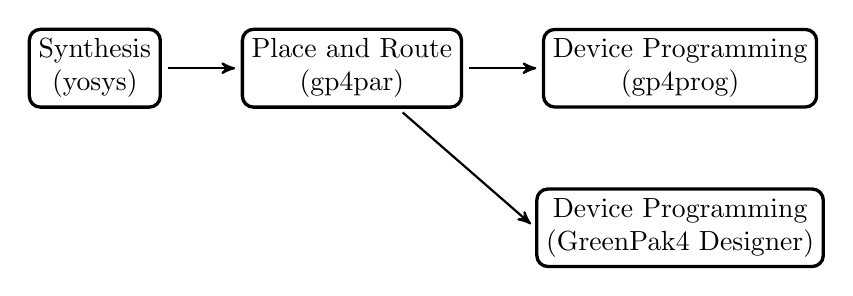
\begin{tikzpicture}[node distance=1cm, auto,]
	\node[box,align=center] (yosys) 
		{Synthesis \\ (yosys)};
	\node[box,align=center,right=of yosys] (gp4par) 
		{Place and Route \\ (gp4par)};
	\node[box,align=center,right=of gp4par] (gp4prog) 
		{Device Programming \\ (gp4prog)};
	\node[box,align=center,right=of gp4par,below=of gp4prog] (gp4vendor) 
		{Device Programming \\ (GreenPak4 Designer)};

	\draw[arrow] (yosys) -- (gp4par);
	\draw[arrow] (gp4par) -- (gp4prog);
	\draw[arrow] (gp4par) -- (gp4vendor.west);
\end{tikzpicture}

 % %nodes
 % \node[punkt] (market) {Market (b)};
 % \node[punkt, inner sep=5pt,below=0.5cm of market]
 % (formidler) {Intermediaries (c)};
 % % We make a dummy figure to make everything look nice.
 % \node[above=of market] (dummy) {};
 % \node[right=of dummy] (t) {Ultimate borrower}
 %   edge[pil,bend left=45] (market.east) % edges are used to connect two nodes
 %   edge[pil, bend left=45] (formidler.east); % .east since we want
 %                                             % consistent style
 % \node[left=of dummy] (g) {Ultimate lender}
 %   edge[pil, bend right=45] (market.west)
 %   edge[pil, bend right=45] (formidler.west)
 %   edge[pil,<->, bend left=45] node[auto] {Direct (a)} (t);

\caption{Data flow between toolchain components}
\label{flow}
\end{figure}

\namestyle{gp4par} is being developed in tandem with \namestyle{GreenPak} support in \namestyle{Yosys}. Most of the \namestyle{GreenPak} features are only available in
the latest development version of \namestyle{Yosys} and have not made it into a stable release yet. We recommend use of the latest
\namestyle{Yosys} from GitHub for testing.

\subsection{Synthesis Example}

A simple synthesis script for \namestyle{Yosys} is shown in figure \ref{yscript}. The script synthesizes a single 
Verilog source file \texttt{Blinky.v}, with a top-level module \texttt{BlinkyTop}, to the netlist \texttt{Blinky.json} 
and targets the \namestyle{SLG46620V}. This script is only a starting point and may be customized as needed. This 
document does not cover synthesis commands; please see the online documentation for \namestyle{Yosys} for command 
documentation.

\begin{figure}[h]
\begin{lstlisting}[language=sh]
#!/usr/bin/env yosys
read_verilog Blinky.v
synth_greenpak4 -top BlinkyTop -part SLG46620V -json Blinky.json
\end{lstlisting}
\caption{Example synthesis script}
\label{yscript}
\end{figure}

\pagebreak
\section{\namestyle{gp4par} Limitations}

The following legal Verilog-2001 features are not supported by \namestyle{gp4par} as of this writing:

\begin{itemize}
\item \whenstyle{Non-scalar top-level module ports}\\All ports on top-level modules must be one bit wide, since there 
is currently no supported syntax for constraining them to package pins. Vector nets may be used at lower levels of the 
hierarchy without restriction.
\end{itemize}

The following \namestyle{SLG46620V} device features are not supported by \namestyle{gp4par} as of this writing:

\begin{itemize}
\item Storage elements: latch mode
\item Counters: Delay, edge detector, PWM, wake-sleep mode, counter cascading.
All clock sources other than on-chip oscillator. Pre-divider value of 12.
\item Voltage reference: DAC, divided Vdd, external references
\item Comparators: Global buffer bandwidth selection, speed doubler
\item ADC
\item DAC
\item PGEN mode of LUT4/PGEN block
\item Wake-Sleep
\item DCMP/PWM
\item Programmble delay line / edge detector
\item Slave SPI
\item Pin 8 reset output
\end{itemize}

\pagebreak
\section{\namestyle{gp4par} HDL Constraints}

There is only one supported constraint entry format at this time, Verilog attributes. There is currently no support for
adding constraints to netlist entities via external constraint files or command line arguments. The general format of a
constraint with name \tokenstyle{FOO} and value 42 applied to the register \wirestyle{foobar} is shown in Figure
\ref{constraint}.

\begin{figure}[h]
\begin{lstlisting}
(* FOO=42 *)
reg[3:0] foobar = 0;
\end{lstlisting}
\caption{Example Verilog attribute constraint}
\label{constraint}
\end{figure}

%%%%%%%%%%%%%%%%%%%%%%%%%%%%%%%%%%%%%%%%%%%%%%%%%%%%%%%%%%%%%%%%%%%%%%%%%%%%%%%%%%%%%%%%%%%%%%%%%%%%%%%%%%%%%%%%%%%%%%%%
% COUNT_EXTRACT

\pagebreak
\subsection{Counter Extraction (\tokenstyle{COUNT\_EXTRACT})}
\label{count-extract}

The \tokenstyle{COUNT\_EXTRACT} constraint controls inference of \tokenref{GP\_COUNT8}{gp-count8} and \tokenref{GP\_COUNT14}{gp-count14} cells from behavioral Verilog. It can be
used to ensure that a given counter in behavioral logic will, or will not, be mapped to a hard macro.

\subsubsection{Applicable Elements}
The \tokenstyle{COUNT\_EXTRACT} constraint may only be used on vector registers.

\subsubsection{Constraint Values}
\begin{itemize}
\item \whenstyle{Vector register}\\
One of the following:
\begin{itemize}
\item \strexamplestyle{AUTO} Same behavior as not specifying any constraint. Counters will be inferred where possible.
\item \strexamplestyle{NO} Do not infer a counter even if the logic matches a supported inference structure.
\item \strexamplestyle{FORCE} Always infer a counter. If a supported inference structure is not found, a synthesis error is produced.
\end{itemize}
\item \whenstyle{Other} \\
This constraint will be silently ignored if used on any other entity.
\end{itemize}

\subsubsection{Verilog Usage Example}

Figure \ref{constraint-count-extract} is an example of a 5-bit down counter with a positive level triggered reset,
configured to force counter inference.

\begin{figure}[h]
\begin{lstlisting}
(* COUNT_EXTRACT = "FORCE" *)
reg[4:0] count = COUNT_MAX;
wire out = (count == 0);
always @(posedge clk, posedge count_rst) begin

	//level triggered reset
	if(count_rst)
		count		<= 0;

	//counter
	else begin

		if(count == 0)
			count	<= COUNT_MAX;
		else
			count	<= count - 1'd1;

	end

end
\end{lstlisting}
\caption{Example for \tokenstyle{COUNT\_EXTRACT} constraint}
\label{constraint-count-extract}
\end{figure}

%%%%%%%%%%%%%%%%%%%%%%%%%%%%%%%%%%%%%%%%%%%%%%%%%%%%%%%%%%%%%%%%%%%%%%%%%%%%%%%%%%%%%%%%%%%%%%%%%%%%%%%%%%%%%%%%%%%%%%%%
% Drive strength

\pagebreak
\subsection{Drive Strength (\tokenstyle{DRIVE\_STRENGTH})}

The \tokenstyle{DRIVE\_STRENGTH} constraint configures the output drive strength on the specified I/O pin. Drive strength refers to current sourcing or sinking capacity.

\subsubsection{Applicable Elements}
The \tokenstyle{DRIVE\_STRENGTH} constraint may only be used on top-level module ports.

\subsubsection{Constraint Values}
\begin{itemize}
\item \whenstyle{Top-level module port (IOB)}
	\begin{itemize}
		\item \strexamplestyle{1X} Default drive strength. This is the default if no constraint is specified.
		\item \strexamplestyle{2X} Two times as strong as the default drive strength.
		\item \strexamplestyle{4X} Four times as strong as the default drive strength.
	\end{itemize}
\item \whenstyle{Other} \\
This constraint may not be used on any other entity.
\end{itemize}

\subsubsection{Verilog Usage Example}

Figure \ref{constraint-drivestrength} is an example of a top-level module with two ports \wirestyle{a} and \wirestyle{b}. Port \wirestyle{a} has 1X drive strength (the default) and port \wirestyle{b} has 2X drive strength.

\begin{figure}[h]
\begin{lstlisting}
module Foo(a, b);

	(* DRIVE_STRENGTH = "1X" *)
	output wire a;

	(* DRIVE_STRENGTH = "2X" *)
	output wire b;

endmodule
\end{lstlisting}
\caption{Example for \tokenstyle{DRIVE\_STRENGTH} constraint}
\label{constraint-drivestrength}
\end{figure}

%%%%%%%%%%%%%%%%%%%%%%%%%%%%%%%%%%%%%%%%%%%%%%%%%%%%%%%%%%%%%%%%%%%%%%%%%%%%%%%%%%%%%%%%%%%%%%%%%%%%%%%%%%%%%%%%%%%%%%%%
% Drive type

\pagebreak
\subsection{Drive Type (\tokenstyle{DRIVE\_TYPE})}

The \tokenstyle{DRIVE\_TYPE} constraint configures the output driver on the specified I/O pin.

\subsubsection{Applicable Elements}
The \tokenstyle{DRIVE\_TYPE} constraint may only be used on top-level module ports.

\subsubsection{Constraint Values}
\begin{itemize}
\item \whenstyle{Top-level module port (IOB)}
	\begin{itemize}
		\item \strexamplestyle{NMOS\_OD} Open drain NMOS (pull-down only) driver.
		\item \strexamplestyle{PMOS\_OD} Open drain PMOS (pull-up only) driver.
		\item \strexamplestyle{PUSHPULL} CMOS digital push-pull driver. This is the default if no constraint is specified.
	\end{itemize}
\item \whenstyle{Other} \\
This constraint may not be used on any other entity.
\end{itemize}

\subsubsection{Verilog Usage Example}

Figure \ref{constraint-drivetype} is an example of a top-level module with two ports \wirestyle{a} and \wirestyle{b}. Port \wirestyle{a} has a push-pull driver and port \wirestyle{b} has an open-drain NMOS driver.

\begin{figure}[h]
\begin{lstlisting}
module Foo(a, b);

	(* DRIVE_TYPE = "PUSHPULL" *)
	output wire a;

	(* DRIVE_TYPE = "NMOS_OD" *)
	output wire b;

endmodule
\end{lstlisting}
\caption{Example for \tokenstyle{DRIVE\_TYPE} constraint}
\label{constraint-drivetype}
\end{figure}

%%%%%%%%%%%%%%%%%%%%%%%%%%%%%%%%%%%%%%%%%%%%%%%%%%%%%%%%%%%%%%%%%%%%%%%%%%%%%%%%%%%%%%%%%%%%%%%%%%%%%%%%%%%%%%%%%%%%%%%%
% Input buffer type

\pagebreak
\subsection{Input Buffer Type (\tokenstyle{IBUF\_TYPE})}

The \tokenstyle{IBUF\_TYPE} constraint configures the input buffer on the specified I/O pin.

\subsubsection{Applicable Elements}
The \tokenstyle{IBUF\_TYPE} constraint may only be used on top-level module ports.

\subsubsection{Constraint Values}
\begin{itemize}
\item \whenstyle{Top-level module port (IOB)}
	\begin{itemize}
		\item \strexamplestyle{ANALOG} Analog buffer for mixed signal hard IP. Note that analog \emph{outputs} must use this setting
		to disable the digital input buffer and ensure correct device operation.
		\item \strexamplestyle{LOW\_VOLTAGE} Low voltage threshold (see datasheet for exact value)
		\item \strexamplestyle{NORMAL} Standard threshold (see datasheet for exact value)
	\end{itemize}
\item \whenstyle{Other} \\
This constraint may not be used on any other entity.
\end{itemize}

\subsubsection{Verilog Usage Example}

Figure \ref{constraint-ibuftype} shows an example of how to configure a top level module input for analog signals.

\begin{figure}[h]
\begin{lstlisting}
(* LOC = "P6" *)
(* IBUF_TYPE = "ANALOG" *)
input wire vin;
\end{lstlisting}
\caption{Example for \tokenstyle{IBUF\_TYPE} constraint}
\label{constraint-ibuftype}
\end{figure}

%%%%%%%%%%%%%%%%%%%%%%%%%%%%%%%%%%%%%%%%%%%%%%%%%%%%%%%%%%%%%%%%%%%%%%%%%%%%%%%%%%%%%%%%%%%%%%%%%%%%%%%%%%%%%%%%%%%%%%%%
% LOC

\pagebreak
\subsection{Physical Location (\tokenstyle{LOC})}

The \tokenstyle{LOC} constraint instructs \namestyle{gp4par} to place the constrained entity at a specific physical
site of the device. This is most commonly used to lock IOBs to specific pins on the package, however advanced users can 
use it to force arbitrary logic to use specific device resources.

The specified location must be valid for the entity being constrained. Attempting to constrain a cell to an illegal 
site causes the initial placement to fail with an error message. For example, figure \ref{invalid-loc} shows the 
results of attempting to constrain a 3-input combinatorial expression to a 2LUT site.

\begin{figure}[h]
\begin{lstlisting}[language=c]
ERROR: Cell $abc$104$auto$blifparse.cc:347:parse_blif$106 has invalid LOC
constraint LUT2_0 (site is of type GP_2LUT, instance is of type GP_3LUT)
\end{lstlisting}
\caption{Error message produced by invalid \tokenstyle{LOC} constraint}
\label{invalid-loc}
\end{figure}

\subsubsection{Applicable Elements}

\begin{itemize}

\item IOBs may be constrained by placing a \tokenstyle{LOC} constraint on the top-level module port declaration.

\item Inferred LUTs and flipflops may be constrained by placing a \tokenstyle{LOC} constraint on the net driven by the 
entity to be constrained. This technique cannot constrain inferred multiple-bit registers or inferred 
combinatorial logic with multiple levels of LUTs; these must be broken up or replaced with primitive instantiation.

\item Instantiated primitives may be constrained by placing a \tokenstyle{LOC} constraint on the primitive declaration 
OR on any net driven by the primitive. Multiple \tokenstyle{LOC} constraints with the same value are ignored; if 
multiple \tokenstyle{LOC} constraints with different values apply to the same element placement will fail with an error 
message (figure \ref{conflicting-loc}).

\item The \tokenstyle{LOC} constraint cannot be applied to inferred counters or shift registers. This will be fixed in 
a future software release.

\end{itemize}

\begin{figure}[h]
\begin{lstlisting}[language=c]
ERROR: Multiple conflicting LOC constraints (COUNT8_5, COUNT8_4) are
attached to cell "lfosc_cnt". Please remove one or more of the constraints
to allow the design to be placed.
\end{lstlisting}
\caption{Error message produced by invalid \tokenstyle{LOC} constraint}
\label{conflicting-loc}
\end{figure}

\pagebreak
\subsubsection{Constraint Values}
\begin{itemize}
\item \whenstyle{\tokenref{Analog comparator}{gp-acmp}}\\
\strvaluestyle{ACMP\_n} where \tokenstyle{n} is the comparator number. Example: \strvaluestyle{ACMP\_2}.
\item \whenstyle{\tokenref{Counter}{gp-count8}}\\
\strvaluestyle{COUNTm\_n} where \tokenstyle{m} is the counter depth and \tokenstyle{n} is the counter number.
Example: \strvaluestyle{COUNT8\_5}.
\item \whenstyle{\tokenref{Flipflop}{gp-dff} (DFF cell or inferred 1-bit register)}\\
\strvaluestyle{DFF\_n} where \tokenstyle{n} is the flipflop number. Example: \strvaluestyle{DFF\_5}.
\item \whenstyle{\tokenref{IOB}{gp-iobuf} (top-level module port or IOB primitive)}\\
\strvaluestyle{Pn} where \tokenstyle{n} is the pin number of the device. Example: \strvaluestyle{P3}.
\item \whenstyle{\tokenref{LUT}{gp-2lut}}\\
\strvaluestyle{LUTm\_n} where \tokenstyle{m} is the number of inputs for the LUT and \tokenstyle{n} is the LUT number.
Example: \strvaluestyle{LUT3\_0}. Note that it is legal to constrain a smaller LUT to a larger site (but not vice 
versa); for example a 2-input function may be constrained to a 3LUT or 4LUT site.
\item \whenstyle{\tokenref{Inverter}{gp-inv}}\\
\strvaluestyle{INV\_n} where \tokenstyle{n} is the number of matrix the inverter is located in. Example:
\strvaluestyle{INV\_0}.
\item \whenstyle{\tokenref{Shift register}{gp-shreg}}\\
\strvaluestyle{SHREG\_n} where \tokenstyle{n} is the number of matrix the shift register is located in. 
Example: \strvaluestyle{SHREG\_0}.
\item \whenstyle{\tokenref{Voltage reference}{gp-vref}}\\
\strvaluestyle{VREF\_n} where \tokenstyle{n} is the number of the attached comparator. Example: 
\strvaluestyle{VREF\_2}.
\item \whenstyle{Other} \\
While this constraint is legal to use on primitives that only have one instance in the device, this is redundant so the 
names of these sites are not documented here (although they may be obtained from the placement report).
\end{itemize}

\pagebreak
\subsubsection{Verilog Usage Example}

Figure \ref{constraint-loc} is an example of a top-level module with four ports \wirestyle{a}, \wirestyle{b},
\wirestyle{o}, and \wirestyle{p}. These ports are constrained to package pins 20, 19, 18, and 17 respectively.

Signal \wirestyle{o} is driven by the inferred register \wirestyle{o\_int}, which is constrained to D flipflop
number 5. Note that \wirestyle{o} could not be directly declared as \tokenstyle{output reg} because this infers both a 
DFF and IOB cell with the same net name. The attached LOC attribute would then apply to the IOB cell and not the DFF.

Signal \wirestyle{p} is driven by the inferred LUT \wirestyle{p\_int}, which is constrained to 3-input LUT number 0 
(rather than one of the 2-input LUTs, as would normally be the case). As with \wirestyle{o}, a separate named net is 
required in this case in order to avoid inferring both an IOB and LUT with ambiguous constraints.

\begin{figure}[h]
\begin{lstlisting}
module Foo(a, b, o, p);

	(* LOC = "P20" *)
	input wire a;

	(* LOC = "P19" *)
	input wire b;

	(* LOC = "P18" *)
	output wire o;
	
	(* LOC = "P17" *)
	output wire p;
	
	(* LOC = "DFF_5" *)
	reg o_int = 0;
	
	assign o = o_int;
	
	(* LOC = "LUT3_0" *)
	wire p_int = (a & b);
	
	assign p = p_int;

endmodule
\end{lstlisting}
\caption{Example for \tokenstyle{LOC} constraint}
\label{constraint-loc}
\end{figure}

%%%%%%%%%%%%%%%%%%%%%%%%%%%%%%%%%%%%%%%%%%%%%%%%%%%%%%%%%%%%%%%%%%%%%%%%%%%%%%%%%%%%%%%%%%%%%%%%%%%%%%%%%%%%%%%%%%%%%%%%
% Pulldown

\clearpage
\pagebreak
\subsection{Pull-Down Resistor (\tokenstyle{PULLDOWN})}

The \tokenstyle{PULLDOWN} constraint instructs \namestyle{gp4par} to enable the pull-down resistor on the specified input. The exact resistor
value ranges may be found in the device datasheet.

\subsubsection{Applicable Elements}
The \tokenstyle{PULLDOWN} constraint may only be used on top-level module ports.

\subsubsection{Constraint Values}
\begin{itemize}
\item \whenstyle{Top-level module port (IOB)}\\
Text string \strvaluestyle{10k}, \strvaluestyle{100k}, or \strvaluestyle{1M}, case sensitive, to specify the nominal value of the pull-down resistor.
\item \whenstyle{Other} \\
This constraint may not be used on any other entity.
\end{itemize}

\subsubsection{Verilog Usage Example}

Figure \ref{constraint-pulldown} is an example of a top-level module with three ports \wirestyle{a}, \wirestyle{b}, and
\wirestyle{o}. Ports \wirestyle{a} and \wirestyle{b} have 10k$\Omega$ pull-down resistors; port \wirestyle{o} is floating.

\begin{figure}[h]
\begin{lstlisting}
module Foo(a, b, o);

	(* PULLDOWN = "10k" *)
	input wire a;

	(* PULLDOWN = "10k" *)
	input wire b;

	input wire o;

endmodule
\end{lstlisting}
\caption{Example for \tokenstyle{PULLDOWN} constraint}
\label{constraint-pulldown}
\end{figure}

%%%%%%%%%%%%%%%%%%%%%%%%%%%%%%%%%%%%%%%%%%%%%%%%%%%%%%%%%%%%%%%%%%%%%%%%%%%%%%%%%%%%%%%%%%%%%%%%%%%%%%%%%%%%%%%%%%%%%%%%
% Pullup

\pagebreak
\subsection{Pull-Up Resistor (\tokenstyle{PULLUP})}

The \tokenstyle{PULLUP} constraint instructs \namestyle{gp4par} to enable the pull-up resistor on the specified input. The exact resistor
value ranges may be found in the device datasheet.

\subsubsection{Applicable Elements}
The \tokenstyle{PULLUP} constraint may only be used on top-level module ports.

\subsubsection{Constraint Values}
\begin{itemize}
\item \whenstyle{Top-level module port (IOB)}\\
Text string \strvaluestyle{10k}, \strvaluestyle{100k}, or \strvaluestyle{1M}, case sensitive, to specify the nominal value of the pull-up resistor.
\item \whenstyle{Other} \\
This constraint may not be used on any other entity.
\end{itemize}

\subsubsection{Verilog Usage Example}

Figure \ref{constraint-pullup} is an example of a top-level module with three ports \wirestyle{a}, \wirestyle{b}, and
\wirestyle{o}. Ports \wirestyle{a} and \wirestyle{b} have 10k$\Omega$ pull-up resistors; port \wirestyle{o} is floating.

\begin{figure}[h]
\begin{lstlisting}
module Foo(a, b, o);

	(* PULLUP = "10k" *)
	input wire a;

	(* PULLUP = "10k" *)
	input wire b;

	input wire o;

endmodule
\end{lstlisting}
\caption{Example for \tokenstyle{PULLUP} constraint}
\label{constraint-pullup}
\end{figure}

%%%%%%%%%%%%%%%%%%%%%%%%%%%%%%%%%%%%%%%%%%%%%%%%%%%%%%%%%%%%%%%%%%%%%%%%%%%%%%%%%%%%%%%%%%%%%%%%%%%%%%%%%%%%%%%%%%%%%%%%
% Schmitt Trigger

\pagebreak
\subsection{Schmitt Trigger (\tokenstyle{SCHMITT\_TRIGGER})}

The \tokenstyle{SCHMITT\_TRIGGER} constraint instructs \namestyle{gp4par} to enable the Schmitt trigger on the specified input. The level
of hysterisis provided may be found in the device datasheet.

\subsubsection{Applicable Elements}
The \tokenstyle{SCHMITT\_TRIGGER} constraint may only be used on top-level module ports configured in bidirectional or input mode.

\subsubsection{Constraint Values}
\begin{itemize}
\item \whenstyle{Top-level module port (IOB)}\\
Specify integer \valuestyle{1} or no value to enable the Schmitt trigger. Specify integer \valuestyle{0}, or no
constraint, to disable it.
\item \whenstyle{Other} \\
This constraint may not be used on any other entity.
\end{itemize}

\subsubsection{Verilog Usage Example}

Figure \ref{constraint-schmitt} is an example of a top-level module with three ports \wirestyle{a}, \wirestyle{b}, and
\wirestyle{o}. The Schmitt trigger is enabled for ports  \wirestyle{a} and \wirestyle{b}, but not \wirestyle{o}.

\begin{figure}[h]
\begin{lstlisting}
module Foo(a, b, o);

	(* SCHMITT_TRIGGER = 1 *)
	input wire a;

	(* SCHMITT_TRIGGER *)
	input wire b;

	(* SCHMITT_TRIGGER = 0 *)
	input wire o;

endmodule
\end{lstlisting}
\caption{Example for \tokenstyle{SCHMITT\_TRIGGER} constraint}
\label{constraint-schmitt}
\end{figure}

%%%%%%%%%%%%%%%%%%%%%%%%%%%%%%%%%%%%%%%%%%%%%%%%%%%%%%%%%%%%%%%%%%%%%%%%%%%%%%%%%%%%%%%%%%%%%%%%%%%%%%%%%%%%%%%%%%%%%%%%
% SHREG_EXTRACT

\pagebreak
\subsection{Shift Register Extraction (\tokenstyle{SHREG\_EXTRACT}) (NOT IMPLEMENTED)}
\label{shreg-extract}

The \tokenstyle{SHREG\_EXTRACT} constraint controls inference of \tokenref{GP\_SHREG}{gp-shreg} cells from behavioral Verilog. It can be
used to ensure that a given shift register in behavioral logic will, or will not be, mapped to a hard macro.

\subsubsection{Applicable Elements}
The \tokenstyle{SHREG\_EXTRACT} constraint may only be used on 1-bit registers.

\subsubsection{Constraint Values}
\begin{itemize}
\item \whenstyle{Single-bit register}\\
One of the following:
\begin{itemize}
\item \strexamplestyle{AUTO} Same behavior as not specifying any constraint. Shift registers will be inferred where possible.
\item \strexamplestyle{NO} Do not infer a shift register even if the logic matches a supported inference structure.
\item \strexamplestyle{FORCE} Always infer a shift register. If a supported inference structure is not found, a synthesis error is produced.
\end{itemize}
\item \whenstyle{Other} \\
This constraint will be silently ignored if used on any other entity.
\end{itemize}

\subsubsection{Verilog Usage Example}

Figure \ref{constraint-shreg-extract} is an example of FIXME

\begin{figure}[h]
\begin{lstlisting}
FIXME
\end{lstlisting}
\caption{Example for \tokenstyle{SHREG\_EXTRACT} constraint}
\label{constraint-shreg-extract}
\end{figure}

%%%%%%%%%%%%%%%%%%%%%%%%%%%%%%%%%%%%%%%%%%%%%%%%%%%%%%%%%%%%%%%%%%%%%%%%%%%%%%%%%%%%%%%%%%%%%%%%%%%%%%%%%%%%%%%%%%%%%%%%
% Timing constraints

\pagebreak
\section{\namestyle{gp4par} Timing Constraints}

Static timing analysis is not yet implemented, thus this section is currently blank.

%%%%%%%%%%%%%%%%%%%%%%%%%%%%%%%%%%%%%%%%%%%%%%%%%%%%%%%%%%%%%%%%%%%%%%%%%%%%%%%%%%%%%%%%%%%%%%%%%%%%%%%%%%%%%%%%%%%%%%%%
% Coding Techniques

\pagebreak
\section{\namestyle{gp4par} HDL Coding Techniques}

When possible, we recommend inferring design elements to maximize design portability. In some cases, such as for hard
IP blocks or when exact control over synthesis results is required, it may be necessary to manually instantiate device
primitives.

%%%%%%%%%%%%%%%%%%%%%%%%%%%%%%%%%%%%%%%%%%%%%%%%%%%%%%%%%%%%%%%%%%%%%%%%%%%%%%%%%%%%%%%%%%%%%%%%%%%%%%%%%%%%%%%%%%%%%%%%
% Counters

\subsection{Counters}

\namestyle{Yosys} provides limited inference capability for counters which match the capabilities of the hard macro counters
(\tokenref{GP\_COUNT8}{gp-count8} and \tokenref{GP\_COUNT14}{gp-count14}) in the device.

Some hard macro capabilities (most notably input dividers) are not yet supported for inference; if these capabilities
are required then use explicit primitive instantiation. Future software releases will expand the set of counter
features which may be inferred.

\subsubsection{Inference Requirements}

In order to be inferred, a counter must:

\begin{itemize}
\item Be less than 14 bits in width
\item Count down only
\item Be initialized to the same (maximum) value by both underflow and by power-on reset
\item Have either no reset, or a positive level triggered reset to zero
\item Not have any logic use the internal counter register. Only the ``underflow" signal may be used by surrounding logic.
\end{itemize}

\subsubsection{Counter Related Constraints}

By default, the \tokenstyle{greenpak4\_counters} pass will attempt to infer a counter macro for every counter matching the
requirements. If this is not desired, use the \tokenref{COUNT\_EXTRACT}{count-extract} constraint to control
inference behavior.

\subsubsection{Verilog Usage Example}

The example in Figure \ref{gp-countinfer-example} shows an example of how to infer a resettable down counter.

\begin{figure}[h]
\begin{lstlisting}
localparam COUNT_MAX = 31;
reg[4:0] count = COUNT_MAX;
wire underflow_out = (count == 0);
always @(posedge clk, posedge count_rst) begin
	if(count_rst)
		count			<= 0;

	else begin
		if(count == 0)
			count		<= COUNT_MAX;
		else
			count		<= count - 1'd1;
	end
end
\end{lstlisting}
\caption{Example for counter inference}
\label{gp-countinfer-example}
\end{figure}

\subsubsection{Reporting}

In order to determine whether a given counter was extracted, look at the synthesis report. Figure
\ref{counter-extraction} shows an example synthesis report with a single inferred counter.

\begin{figure}[h]
{\small
\begin{verbatim}
2.7.
Executing GREENPAK4_COUNTERS pass (mapping counters to hard IP blocks).
  Found 3-bit non-resettable down counter (from 7) for register count
    declared at Blinky.v:93
Extracted 1 counters
\end{verbatim}
}
\caption{Sample extraction report}
\label{counter-extraction}
\end{figure}

%%%%%%%%%%%%%%%%%%%%%%%%%%%%%%%%%%%%%%%%%%%%%%%%%%%%%%%%%%%%%%%%%%%%%%%%%%%%%%%%%%%%%%%%%%%%%%%%%%%%%%%%%%%%%%%%%%%%%%%%
% Shift Registers

\pagebreak
\subsection{Shift Registers}

\namestyle{Yosys} provides inference capability for shift registers matching the capabilities of the ``pipe delay" block in the
\namestyle{SLG46620/21}. The shift register is automatically initialized to zero at power-up; there is no support for initializing
to any other value.

The internal inverter is not yet supported for inference. If this is required for your design, consider manual
instantiation of a \tokenref{GP\_SHREG}{gp-shreg} primitive.

\subsubsection{Inference Requirements}

In order to be inferred as a single \tokenref{GP\_SHREG}{gp-shreg} primitive, a shift register must:

\begin{itemize}
\item Be at most 16 bits in depth
\item Be initialized to zero, or uninitialized
\item Have either no reset, or a positive level triggered reset to zero
\item Have at most two taps in the shift register connected to external logic. If more taps are required, a second
shift register and/or discrete flipflops may be inferred.
\end{itemize}

\subsubsection{Shift Register Related Constraints}

As of now there are no constraints to force or disable inference of shift registers. A constraint analogous to
\tokenref{COUNT\_EXTRACT}{count-extract} will likely be added in a future software release.

\subsubsection{Verilog Usage Example}

The example in Figure \ref{gp-shreginfer-example} shows an example of how to infer a shift register with taps delayed 8
and 16 clocks from the input.

\begin{figure}[h]
\begin{lstlisting}
wire led_in;
reg[15:0] led_shreg = 0;
assign led1 = led_shreg[7];
assign led2 = led_shreg[15];
always @(posedge clk) begin
	led_shreg	<= {led_shreg[14:0], led_in};
end
\end{lstlisting}
\caption{Example for shift register inference}
\label{gp-shreginfer-example}
\end{figure}

\subsubsection{Reporting}

In order to determine whether a given shift register was extracted, look at the synthesis report. Figure
\ref{shreg-extraction} shows an example synthesis report with a single inferred shift register.

\begin{figure}[h]
{\small
\begin{verbatim}
2.15. Executing SHREGMAP pass (map shift registers).
Converting Blinky.$auto$simplemap.cc:373:simplemap_dff$132 ...
  Blinky.$auto$simplemap.cc:373:simplemap_dff$147 to a shift
  register with depth 16.
Converted 16 dff cells into 1 shift registers.
\end{verbatim}
}
\caption{Sample extraction report}
\label{shreg-extraction}
\end{figure}

%%%%%%%%%%%%%%%%%%%%%%%%%%%%%%%%%%%%%%%%%%%%%%%%%%%%%%%%%%%%%%%%%%%%%%%%%%%%%%%%%%%%%%%%%%%%%%%%%%%%%%%%%%%%%%%%%%%%%%%%
% Primitives

\pagebreak
\section{\namestyle{gp4par} Verilog Primitives}

This section lists all of the device-dependent primitives wrapping hard IP blocks in the device. These may be used for
features which are not yet supported by inference, or when exact control over synthesis results is needed.

Pay careful attention to port names and descriptions as these may not exactly match the Silego primitives; some have
been changed in order to allow cleaner and more modular HDL. For example, the single ``oscillator" block is represented
in Verilog by a separate block for each of the three internal oscillators.

%%%%%%%%%%%%%%%%%%%%%%%%%%%%%%%%%%%%%%%%%%%%%%%%%%%%%%%%%%%%%%%%%%%%%%%%%%%%%%%%%%%%%%%%%%%%%%%%%%%%%%%%%%%%%%%%%%%%%%%%
% GP_2LUT

\pagebreak
\subsection{\tokenstyle{GP\_2LUT}: 2-Input Lookup Table}
\label{gp-2lut}

\subsubsection{Introduction}
This primitive corresponds to a single 2-input lookup table. It can implement any combinatorial function of two
inputs and one output.

The LUT output is the \{\tokenstyle{IN1}, \tokenstyle{IN0}\}'th bit of the truth table supplied in the \tokenstyle{INIT} attribute.

This primitive may be manually instantiated if exact control over LUT packing is required, but for most applications we
recommend inferring logic.

Note that the placer may re-map \tokenref{GP\_2LUT}{gp-2lut} primitives to 3- or 4-input LUT sites to reduce routing 
congestion. The \tokenref{LOC}{LOC} constraint may be used to force the primitive to a specific 2-input LUT if 
necessary.

\subsubsection{Port Descriptions}

\begin{tabularx}{\textwidth}{lllX}
\thinhline
\whenstyle{Port} & \whenstyle{Type} & \whenstyle{Width} & \whenstyle{Function} \\
\thickhline
\tokenstyle{IN0} & Input & 1 & Least significant input bit. \\
\thinhline
\tokenstyle{IN1} & Input & 1 & Input bit. \\
\thinhline
\tokenstyle{OUT} & Output & 1 & Lookup table output. \\
\thinhline
\end{tabularx}

\subsubsection{Parameter Descriptions}

\begin{tabularx}{\textwidth}{lllX}
\thinhline
\whenstyle{Parameter} & \whenstyle{Type} & \whenstyle{Width} & \whenstyle{Function} \\
\thickhline
\tokenstyle{INIT} & Integer & 4 & LUT truth table. \\
\thinhline
\end{tabularx}

\subsubsection{Verilog Usage Example}

The example shown in figure \ref{gp-2LUT-example} sets \wirestyle{o} to the bitwise AND of \wirestyle{a} and \wirestyle{b}.

\begin{figure}[h]
\begin{lstlisting}
wire a;
wire b;
wire o;
GP_2LUT #(
	.INIT(4'h4)
) lut(
	.IN0(a),
	.IN1(b),
	.OUT(o)
);
\end{lstlisting}
\caption{Example usage of \tokenstyle{GP\_2LUT}}
\label{gp-2LUT-example}
\end{figure}

%%%%%%%%%%%%%%%%%%%%%%%%%%%%%%%%%%%%%%%%%%%%%%%%%%%%%%%%%%%%%%%%%%%%%%%%%%%%%%%%%%%%%%%%%%%%%%%%%%%%%%%%%%%%%%%%%%%%%%%%
% GP_3LUT

\pagebreak
\subsection{\tokenstyle{GP\_3LUT}: 3-Input Lookup Table}
\label{gp-3lut}

\subsubsection{Introduction}
This primitive corresponds to a single 3-input lookup table. It can implement any combinatorial function of three
inputs and one output.

The LUT output is the \{\tokenstyle{IN2}, \tokenstyle{IN1}, \tokenstyle{IN0}\}'th bit of the truth table supplied in the \tokenstyle{INIT} attribute.

This primitive may be manually instantiated if exact control over LUT packing is required, but for most applications we
recommend inferring logic.

Note that the placer may re-map \tokenref{GP\_3LUT}{gp-3lut} primitives to 4-input LUT sites to reduce routing 
congestion. The \tokenref{LOC}{LOC} constraint may be used to force the primitive to a specific 3-input LUT if 
necessary.

\subsubsection{Port Descriptions}

\begin{tabularx}{\textwidth}{lllX}
\thinhline
\whenstyle{Port} & \whenstyle{Type} & \whenstyle{Width} & \whenstyle{Function} \\
\thickhline
\tokenstyle{IN0} & Input & 1 & Least significant input bit. \\
\thinhline
\tokenstyle{IN1} & Input & 1 & Input bit. \\
\thinhline
\tokenstyle{IN2} & Input & 1 & Most significant input bit. \\
\thinhline
\tokenstyle{OUT} & Output & 1 & Lookup table output. \\
\thinhline
\end{tabularx}

\subsubsection{Parameter Descriptions}

\begin{tabularx}{\textwidth}{lllX}
\thinhline
\whenstyle{Parameter} & \whenstyle{Type} & \whenstyle{Width} & \whenstyle{Function} \\
\thickhline
\tokenstyle{INIT} & Integer & 8 & LUT truth table. \\
\thinhline
\end{tabularx}

\subsubsection{Verilog Usage Example}

The example shown in figure \ref{gp-3LUT-example} sets \wirestyle{o} to the bitwise AND of \wirestyle{a}, \wirestyle{b}, and \wirestyle{c}.

\begin{figure}[h]
\begin{lstlisting}
wire a;
wire b;
wire c;
wire o;
GP_3LUT #(
	.INIT(8'h80)
) lut(
	.IN0(a),
	.IN1(b),
	.IN2(c),
	.OUT(o)
);
\end{lstlisting}
\caption{Example usage of \tokenstyle{GP\_3LUT}}
\label{gp-3LUT-example}
\end{figure}

%%%%%%%%%%%%%%%%%%%%%%%%%%%%%%%%%%%%%%%%%%%%%%%%%%%%%%%%%%%%%%%%%%%%%%%%%%%%%%%%%%%%%%%%%%%%%%%%%%%%%%%%%%%%%%%%%%%%%%%%
% GP_4LUT

\pagebreak
\subsection{\tokenstyle{GP\_4LUT}: 4-Input Lookup Table}
\label{gp-4lut}

\subsubsection{Introduction}
This primitive corresponds to a single 4-input lookup table. It can implement any combinatorial function of four
inputs and one output.

The LUT output is the \{\tokenstyle{IN3}, \tokenstyle{IN2}, \tokenstyle{IN1}, \tokenstyle{IN0}\}'th bit of the truth table supplied in the \tokenstyle{INIT} attribute.

This primitive may be manually instantiated if exact control over LUT packing is required, but for most applications we
recommend inferring logic.

\subsubsection{Port Descriptions}

\begin{tabularx}{\textwidth}{lllX}
\thinhline
\whenstyle{Port} & \whenstyle{Type} & \whenstyle{Width} & \whenstyle{Function} \\
\thickhline
\tokenstyle{IN0} & Input & 1 & Least significant input bit. \\
\thinhline
\tokenstyle{IN1} & Input & 1 & Input bit. \\
\thinhline
\tokenstyle{IN2} & Input & 1 & Input bit. \\
\thinhline
\tokenstyle{IN3} & Input & 1 & Most significant input bit. \\
\thinhline
\tokenstyle{OUT} & Output & 1 & Lookup table output. \\
\thinhline
\end{tabularx}

\subsubsection{Parameter Descriptions}

\begin{tabularx}{\textwidth}{lllX}
\thinhline
\whenstyle{Parameter} & \whenstyle{Type} & \whenstyle{Width} & \whenstyle{Function} \\
\thickhline
\tokenstyle{INIT} & Integer & 16 & LUT truth table. \\
\thinhline
\end{tabularx}

\subsubsection{Verilog Usage Example}

The example shown in figure \ref{gp-4LUT-example} sets \wirestyle{o} to the bitwise AND of \wirestyle{a}, \wirestyle{b}, \wirestyle{c},
and \wirestyle{d}.

\begin{figure}[h]
\begin{lstlisting}
wire a;
wire b;
wire c;
wire d;
wire o;
GP_4LUT #(
	.INIT(16'h8000)
) lut(
	.IN0(a),
	.IN1(b),
	.IN2(c),
	.IN3(d)
	.OUT(o)
);
\end{lstlisting}
\caption{Example usage of \tokenstyle{GP\_4LUT}}
\label{gp-4LUT-example}
\end{figure}

%%%%%%%%%%%%%%%%%%%%%%%%%%%%%%%%%%%%%%%%%%%%%%%%%%%%%%%%%%%%%%%%%%%%%%%%%%%%%%%%%%%%%%%%%%%%%%%%%%%%%%%%%%%%%%%%%%%%%%%%
% GP_ABUF

\pagebreak
\subsection{\tokenstyle{GP\_ABUF}: Analog Buffer}
\label{gp-abuf}

\subsubsection{Introduction}
This primitive represents an analog buffer which may be used to reduce loading on comparator inputs. Note that not all
comparators have buffers on the input; see device datasheet for details.

\subsubsection{Port Descriptions}

\begin{tabularx}{\textwidth}{lllX}
\thinhline
\whenstyle{Port} & \whenstyle{Type} & \whenstyle{Width} & \whenstyle{Function} \\
\thickhline
\tokenstyle{IN} & Input & 1 & Connect to analog output from IOB.\\
\thinhline
\tokenstyle{OUT} & Output & 1 & Connect to \tokenstyle{VIN} of a \tokenref{GP\_ACMP}{gp-acmp} block.\\
\thinhline
\end{tabularx}

\subsubsection{Parameter Descriptions}

No parameters.

\subsubsection{Verilog Usage Example}

The example shown in figure \ref{gp-abuf-example} buffers the signal \wirestyle{vin} to \wirestyle{vin\_buf}.

\begin{figure}[h]
\begin{lstlisting}
wire vin;
wire vin_buf;
GP_ABUF abuf(
	.IN(vin),
	.OUT(vin_buf)
);
\end{lstlisting}
\caption{Example usage of \tokenstyle{GP\_ABUF}}
\label{gp-abuf-example}
\end{figure}

%%%%%%%%%%%%%%%%%%%%%%%%%%%%%%%%%%%%%%%%%%%%%%%%%%%%%%%%%%%%%%%%%%%%%%%%%%%%%%%%%%%%%%%%%%%%%%%%%%%%%%%%%%%%%%%%%%%%%%%%
% GP_ACMP

\pagebreak
\subsection{\tokenstyle{GP\_ACMP}: Analog Comparator}
\label{gp-acmp}

\subsubsection{Introduction}
This primitive represents an analog comparator.

The comparator may not be powered on until the power-on reset process has completed. The \tokenstyle{PWREN} input must be tied to
either the reset-done output of the \tokenref{GP\_POR}{gp-por} block, or an arbitrary digital expression ANDed with the reset-done output.

\subsubsection{Port Descriptions}

\begin{tabularx}{\textwidth}{lllX}
\thinhline
\whenstyle{Port} & \whenstyle{Type} & \whenstyle{Width} & \whenstyle{Function} \\
\thickhline
\tokenstyle{PWREN} & Input & 1 &
	\whenstyle{When 1:} normal operation \newline
	\whenstyle{When 0:} power down mode. \\
\thinhline
\tokenstyle{OUT} & Output & 1 &
	\whenstyle{1:} when \tokenstyle{VIN} $>$ \tokenstyle{VREF} and comparator is running \newline
	\whenstyle{0:} when \tokenstyle{VIN} $<$ \tokenstyle{VREF} or comparator is powered down. \\
\thinhline
\tokenstyle{VIN} & Input & 1 & Input voltage (Vdd or external analog input from IOB). \\
\thinhline
\tokenstyle{VREF} & Input & 1 & Input reference voltage. \\
\thinhline
\end{tabularx}

\subsubsection{Parameter Descriptions}

\begin{tabularx}{\textwidth}{lllX}
\thinhline
\whenstyle{Parameter} & \whenstyle{Type} & \whenstyle{Width} & \whenstyle{Function} \\
\thickhline
\tokenstyle{BANDWIDTH} & String & N/A &
	Comparator bandwidth. Legal values are \strvaluestyle{LOW} and \strvaluestyle{HIGH}, see device datasheet for actual bandwidth values. \\
\thinhline
\tokenstyle{VIN\_ATTEN} & Integer & 3 &
	Attenuation for the input, represented as inverse gain. Legal values are 1, 2, 3, 4. Note that not all comparators support selectable attenuation, check device datasheet for details.\\
\thinhline
\tokenstyle{VIN\_ISRC\_EN} & Boolean & 1 &
	Set to 1 to enable the $100 \mu A$ current source on the input. Note that not all comparators support the current
	source, check device datasheet for details.\\
\thinhline
\tokenstyle{HYSTERESIS} & Integer & 8 &
	Hysteresis, in mV. Legal values are 0, 25, 50, 200. See device datasheet for offset notes.\\
\thinhline
\end{tabularx}

\subsubsection{Verilog Usage Example}

The example shown in figure \ref{gp-acmp-example} sets cout1 to true if \wirestyle{vin} is greater than \wirestyle{vref\_750}. The comparator is set to have 25 mV of hysteresis and low bandwidth.

\begin{figure}[h]
\begin{lstlisting}
wire por_done;
wire cout1;
wire vin;
wire vref_750;
GP_ACMP #(
	.BANDWIDTH("LOW"),
	.VIN_ATTEN(4'd1),
	.VIN_ISRC_EN(1'b0),
	.HYSTERESIS(8'd25)
) cmp (
	.PWREN(por_done),
	.OUT(cout1),
	.VIN(vin),
	.VREF(vref_750)
);
\end{lstlisting}
\caption{Example usage of \tokenstyle{GP\_ACMP}}
\label{gp-acmp-example}
\end{figure}

%%%%%%%%%%%%%%%%%%%%%%%%%%%%%%%%%%%%%%%%%%%%%%%%%%%%%%%%%%%%%%%%%%%%%%%%%%%%%%%%%%%%%%%%%%%%%%%%%%%%%%%%%%%%%%%%%%%%%%%%
% GP_BANDGAP

\pagebreak
\clearpage
\subsection{\tokenstyle{GP\_BANDGAP}: Bandgap Voltage Reference}

\subsubsection{Introduction}
This primitive allows configuration of the bandgap voltage reference. It produces a 1.0V reference which is used 
internally by the \tokenref{GP\_VREF}{gp-vref} block. (This connection is implicit and does not need to be provided in 
your HDL.)

\subsubsection{Port Descriptions}

\begin{tabularx}{\textwidth}{lllX}
\thinhline
\whenstyle{Port} & \whenstyle{Type} & \whenstyle{Width} & \whenstyle{Function} \\
\thickhline
\tokenstyle{OK} & Output & 1 & Goes high when bandgap voltage reference is stable. \\
\thinhline
\end{tabularx}

\subsubsection{Parameter Descriptions}

\begin{tabularx}{\textwidth}{lllX}
\thinhline
\whenstyle{Parameter} & \whenstyle{Type} & \whenstyle{Width} & \whenstyle{Function} \\
\thickhline
\tokenstyle{AUTO\_PWRDN} & Boolean & 1 &
	\whenstyle{When 1:} Automatically power down bandgap when all loads are powered down. \newline
	\whenstyle{When 0:} Automatic power-down is disabled. \newline The bandgap is always on.\\
\thinhline
\tokenstyle{CHOPPER\_EN} & Boolean & 1 &
	Specify whether to enable the chopper stabilization for the bandgap op-amp. Should always be 1. \\
\thinhline
\tokenstyle{OUT\_DELAY} & Integer & 1 &
	Time, in $\mu s$, to wait after bandgap startup before asserting \tokenstyle{OK}. Legal values are 100 or 550.\\
\thinhline
\end{tabularx}

\subsubsection{Verilog Usage Example}

The example shown in figure \ref{gp-bandgap-example} sets \wirestyle{bg\_ok} high $550 \mu s$ after reset.

\begin{figure}[h]
\begin{lstlisting}
wire bg_ok;
wire bandgap_vout;
GP_BANDGAP #(
	.AUTO_PWRDN(0),
	.CHOPPER_EN(1),
	.OUT_DELAY(550)
) bandgap (
	.OK(bg_ok)
);
\end{lstlisting}
\caption{Example usage of \tokenstyle{GP\_BANDGAP}}
\label{gp-bandgap-example}
\end{figure}

%%%%%%%%%%%%%%%%%%%%%%%%%%%%%%%%%%%%%%%%%%%%%%%%%%%%%%%%%%%%%%%%%%%%%%%%%%%%%%%%%%%%%%%%%%%%%%%%%%%%%%%%%%%%%%%%%%%%%%%%
% GP_COUNT8

\pagebreak
\subsection{\tokenstyle{GP\_COUNT8}: 8-Bit Resettable Down Counter}
\label{gp-count8}

\subsubsection{Introduction}
This primitive represents an 8-bit down counter. The count register is initialized to \tokenstyle{COUNT\_TO} at 
power-on reset, and to 0 by the reset pin.

Note that this primitive does \emph{not} always map to a hard IP block with \emph{exactly} 8 bit depth. The technology
mapper may map \tokenstyle{GP\_COUNT8} cells to unused 14-bit counters in order to relieve routing pressure.
In this case, the high 6 bits of the counter will always be zero.

\subsubsection{Port Descriptions}

\begin{tabularx}{\textwidth}{lllX}
\thinhline
\whenstyle{Port} & \whenstyle{Type} & \whenstyle{Width} & \whenstyle{Function} \\
\thickhline
\tokenstyle{CLK} & Input & 1 & The input clock signal. \\
\thinhline
\tokenstyle{RST} & Input & 1 & Reset input (polarity depends on \tokenstyle{RESET\_MODE}).
	When triggered, resets the count register to zero. \\
\thinhline
\tokenstyle{OUT} & Output & 1 & Counter underflow output. High whenever the count register equals zero. \\
\thinhline
\end{tabularx}

\subsubsection{Parameter Descriptions}

\begin{tabularx}{\textwidth}{lllX}
\thinhline
\whenstyle{Parameter} & \whenstyle{Type} & \whenstyle{Width} & \whenstyle{Function} \\
\thickhline
\tokenstyle{CLKIN\_DIVIDE} & Integer & 8 &
	Input clock divider. Legal values depend on what source \tokenstyle{CLK} is driven by, see device datasheet.\\
\thinhline
\tokenstyle{COUNT\_TO} & Integer & 8 & Value to set the counter to on underflow. \\
\thinhline
\tokenstyle{RESET\_MODE} & String & N/A &
	\strexamplestyle{RISING} Resets the counter on a rising edge of \tokenstyle{RST}. \newline
	\strexamplestyle{FALLING} Resets the counter on a falling edge of \tokenstyle{RST}. \newline
	\strexamplestyle{BOTH} Resets the counter on any edge of \tokenstyle{RST}. \newline
	\strexamplestyle{LEVEL} Resets the counter when \tokenstyle{RST} is high. \\
\thinhline
\end{tabularx}

\subsubsection{Verilog Usage Example}

The example shown in figure \ref{gp-count8-example} begins counting from \datastyle{8'hcc} down to zero,
on rising edges of \wirestyle{clk}, as soon as the device exits power-on reset. When the counter reaches zero 
\wirestyle{underflow} goes high for one \wirestyle{clk} cycle and the counter is reset to \datastyle{8'hcc}. 
The counter also resets immediately to zero, and is held in reset, when \wirestyle{count\_rst} is high.

\begin{figure}[h]
\begin{lstlisting}
wire underflow;
wire count_rst;
wire clk;
GP_COUNT8 #(
	.RESET_MODE("LEVEL"),
	.COUNT_TO(8'hcc),
	.CLKIN_DIVIDE(1)
) lfosc_cnt (
	.CLK(clk),
	.RST(count_rst),
	.OUT(underflow)
);
\end{lstlisting}
\caption{Example usage of \tokenstyle{GP\_COUNT8}}
\label{gp-count8-example}
\end{figure}

%%%%%%%%%%%%%%%%%%%%%%%%%%%%%%%%%%%%%%%%%%%%%%%%%%%%%%%%%%%%%%%%%%%%%%%%%%%%%%%%%%%%%%%%%%%%%%%%%%%%%%%%%%%%%%%%%%%%%%%%
% GP_COUNT8_ADV

\pagebreak
\subsection{\tokenstyle{GP\_COUNT8\_ADV}: 8-Bit Resettable Up/Down Counter With Clock Gating}
\label{gp-count8-adv}

\subsubsection{Introduction}
This primitive represents an 8-bit up/down counter. The count register is initialized to \tokenstyle{COUNT\_TO} at
power-on reset, underflow or overflow, and to a configurable value by the reset pin.

\subsubsection{Port Descriptions}

\begin{tabularx}{\textwidth}{lllX}
\thinhline
\whenstyle{Port} & \whenstyle{Type} & \whenstyle{Width} & \whenstyle{Function} \\
\thickhline
\tokenstyle{CLK} & Input & 1 & The input clock signal. \\
\thinhline
\tokenstyle{RST} & Input & 1 & Reset input (polarity depends on \tokenstyle{RESET\_MODE}). \\
\thinhline
\tokenstyle{UP} & Input & 1 & Direction input. \\
\thinhline
\tokenstyle{KEEP} & Input & 1 & Clock gating input. \\
\thinhline
\tokenstyle{OUT} & Output & 1 & Counter underflow/overflow output. \newline
	\whenstyle{When \tokenstyle{UP} is 0:} High whenever the count register equals zero. \newline
	\whenstyle{When \tokenstyle{UP} is 1:} High whenever the count register equals \datastyle{8'hff}. \\
\thinhline
\end{tabularx}

\subsubsection{Parameter Descriptions}

\begin{tabularx}{\textwidth}{lllX}
\thinhline
\whenstyle{Parameter} & \whenstyle{Type} & \whenstyle{Width} & \whenstyle{Function} \\
\thickhline
\tokenstyle{CLKIN\_DIVIDE} & Integer & 8 &
	Input clock divider. Legal values depend on what source \tokenstyle{CLK} is driven by, see device datasheet.\\
\thinhline
\tokenstyle{COUNT\_TO} & Integer & 8 & Value to set the counter to on underflow. \\
\thinhline
\tokenstyle{RESET\_MODE} & String & N/A &
	\strexamplestyle{RISING} Resets the counter on a rising edge of \tokenstyle{RST}. \newline
	\strexamplestyle{FALLING} Resets the counter on a falling edge of \tokenstyle{RST}. \newline
	\strexamplestyle{BOTH} Resets the counter on any edge of \tokenstyle{RST}. \newline
	\strexamplestyle{LEVEL} Resets the counter when \tokenstyle{RST} is high. \\
\thinhline
\tokenstyle{RESET\_VALUE} & String & N/A &
	\strexamplestyle{COUNT\_TO} Resets the counter to \tokenstyle{COUNT\_TO}. \newline
	\strexamplestyle{ZERO} Resets the counter to 0. \\
\thinhline
\end{tabularx}

\subsubsection{Verilog Usage Example}

The example shown in figure \ref{gp-count8-adv-example} begins counting from \datastyle{8'hcc} up to \datastyle{8'hff}, 
on rising edges of \wirestyle{clk}, as soon as the device exits power-on reset.
When the counter reaches \datastyle{8'hff}, \wirestyle{overflow} goes high for one \wirestyle{clk} cycle and
the counter is reset to \datastyle{8'hcc}. The counter also resets immediately to \datastyle{8'hcc}, and is held
in reset,  when \wirestyle{count\_rst} is high.

\begin{figure}[h]
\begin{lstlisting}
wire clk;
wire count_rst;
wire overflow;
GP_COUNT8_ADV #(
	.CLKIN_DIVIDE(1)
	.COUNT_TO(8'hcc),
	.RESET_MODE("LEVEL"),
	.RESET_VALUE("COUNT_TO"),
) up_cnt (
	.CLK(clk),
	.RST(count_rst),
	.OUT(overflow),
	.UP(1'b1),
	.KEEP(1'b0)
);
\end{lstlisting}
\caption{Example usage of \tokenstyle{GP\_COUNT8\_ADV}}
\label{gp-count8-adv-example}
\end{figure}

%%%%%%%%%%%%%%%%%%%%%%%%%%%%%%%%%%%%%%%%%%%%%%%%%%%%%%%%%%%%%%%%%%%%%%%%%%%%%%%%%%%%%%%%%%%%%%%%%%%%%%%%%%%%%%%%%%%%%%%%
% GP_COUNT14

\pagebreak
\subsection{\tokenstyle{GP\_COUNT14}: 14-Bit Resettable Down Counter}
\label{gp-count14}

\subsubsection{Introduction}
This primitive represents an 14-bit down counter. The count register is initialized to \tokenstyle{COUNT\_TO} at 
power-on reset, and to 0 by the reset pin.

In the current software, this primitive currently will always map to a 14-bit counter cell in the device. A planned
future optimization will allow the technology mapper to map 14-bit counters in the netlist to 8-bit counter cells if
the provided count value is less than 256. This should allow better packing density for parameterizable modules
containing counters of variable depth.

\subsubsection{Port Descriptions}

\begin{tabularx}{\textwidth}{lllX}
\thinhline
\whenstyle{Port} & \whenstyle{Type} & \whenstyle{Width} & \whenstyle{Function} \\
\thickhline
\tokenstyle{CLK} & Input & 1 & The input clock signal. \\
\thinhline
\tokenstyle{RST} & Input & 1 & Reset input (polarity depends on \tokenstyle{RESET\_MODE}). When triggered, resets the count register to zero. \\
\thinhline
\tokenstyle{OUT} & Output & 1 & Counter underflow output. High whenever the count register equals zero. \\
\thinhline
\end{tabularx}

\subsubsection{Parameter Descriptions}

\begin{tabularx}{\textwidth}{lllX}
\thinhline
\whenstyle{Parameter} & \whenstyle{Type} & \whenstyle{Width} & \whenstyle{Function} \\
\thickhline
\tokenstyle{CLKIN\_DIVIDE} & Integer & 8 &
	Input clock divider. Legal values depend on what source \tokenstyle{CLK} is driven by, see device datasheet.\\
\thinhline
\tokenstyle{COUNT\_TO} & Integer & 14 & Value to set the counter to on underflow. \\
\thinhline
\tokenstyle{RESET\_MODE} & String & N/A &
	\strexamplestyle{RISING} Resets the counter on a rising edge of \tokenstyle{RST}. \newline
	\strexamplestyle{FALLING} Resets the counter on a falling edge of \tokenstyle{RST}. \newline
	\strexamplestyle{BOTH} Resets the counter on any edge of \tokenstyle{RST}. \newline
	\strexamplestyle{LEVEL} Resets the counter when \tokenstyle{RST} is high. \\
\thinhline
\end{tabularx}

\subsubsection{Verilog Usage Example}

The example shown in figure \ref{gp-count14-example} begins counting from \datastyle{14'd3141} down to zero, on 
rising edges of \wirestyle{clk}, as soon as the device exits power-on reset. When the counter reaches zero 
\wirestyle{underflow} goes high for one \wirestyle{clk} cycle and the counter is reset to \datastyle{14'd3141}.
The counter also resets immediately to zero, and is held in reset, when \wirestyle{count\_rst} is high.

\begin{figure}[h]
\begin{lstlisting}
wire underflow;
wire count_rst;
wire clk;
GP_COUNT14 #(
	.RESET_MODE("LEVEL"),
	.COUNT_TO(14'd3141),
	.CLKIN_DIVIDE(1)
) lfosc_cnt (
	.CLK(clk),
	.RST(count_rst),
	.OUT(underflow)
);
\end{lstlisting}
\caption{Example usage of \tokenstyle{GP\_COUNT14}}
\label{gp-count14-example}
\end{figure}

%%%%%%%%%%%%%%%%%%%%%%%%%%%%%%%%%%%%%%%%%%%%%%%%%%%%%%%%%%%%%%%%%%%%%%%%%%%%%%%%%%%%%%%%%%%%%%%%%%%%%%%%%%%%%%%%%%%%%%%%
% GP_COUNT14_ADV

\pagebreak
\subsection{\tokenstyle{GP\_COUNT14\_ADV}: 14-Bit Resettable Up/Down Counter With Clock Gating}
\label{gp-count14-adv}

\subsubsection{Introduction}
This primitive represents a 14-bit up/down counter. The count register is initialized to \tokenstyle{COUNT\_TO} at
power-on reset, underflow or overflow, and to a configurable value by the reset pin.

\subsubsection{Port Descriptions}

\begin{tabularx}{\textwidth}{lllX}
\thinhline
\whenstyle{Port} & \whenstyle{Type} & \whenstyle{Width} & \whenstyle{Function} \\
\thickhline
\tokenstyle{CLK} & Input & 1 & The input clock signal. \\
\thinhline
\tokenstyle{RST} & Input & 1 & Reset input (polarity depends on \tokenstyle{RESET\_MODE}). \\
\thinhline
\tokenstyle{UP} & Input & 1 & Direction input. \\
\thinhline
\tokenstyle{KEEP} & Input & 1 & Clock gating input. \\
\thinhline
\tokenstyle{OUT} & Output & 1 & Counter underflow/overflow output. \newline
	\whenstyle{When \tokenstyle{UP} is 0:} High whenever the count register equals zero. \newline
	\whenstyle{When \tokenstyle{UP} is 1:} High whenever the count register equals \datastyle{14'h3fff}. \\
\thinhline
\end{tabularx}

\subsubsection{Parameter Descriptions}

\begin{tabularx}{\textwidth}{lllX}
\thinhline
\whenstyle{Parameter} & \whenstyle{Type} & \whenstyle{Width} & \whenstyle{Function} \\
\thickhline
\tokenstyle{CLKIN\_DIVIDE} & Integer & 8 &
	Input clock divider. Legal values depend on what source \tokenstyle{CLK} is driven by, see device datasheet.\\
\thinhline
\tokenstyle{COUNT\_TO} & Integer & 14 & Value to set the counter to on underflow. \\
\thinhline
\tokenstyle{RESET\_MODE} & String & N/A &
	\strexamplestyle{RISING} Resets the counter on a rising edge of \tokenstyle{RST}. \newline
	\strexamplestyle{FALLING} Resets the counter on a falling edge of \tokenstyle{RST}. \newline
	\strexamplestyle{BOTH} Resets the counter on any edge of \tokenstyle{RST}. \newline
	\strexamplestyle{LEVEL} Resets the counter when \tokenstyle{RST} is high. \\
\thinhline
\tokenstyle{RESET\_VALUE} & String & N/A &
	\strexamplestyle{COUNT\_TO} Resets the counter to \tokenstyle{COUNT\_TO}. \newline
	\strexamplestyle{ZERO} Resets the counter to 0. \\
\thinhline
\end{tabularx}

\subsubsection{Verilog Usage Example}

The example shown in figure \ref{gp-count14-adv-example} begins counting from \datastyle{14'd3141} up to 
\datastyle{14'h3fff}, on rising edges of \wirestyle{clk}, as soon as the device exits power-on reset.
When the counter reaches \datastyle{14'h3fff}, \wirestyle{overflow} goes high for one \wirestyle{clk} cycle and 
the counter is reset to \datastyle{14'd3141}. The counter also resets immediately to \datastyle{14'd0}, and 
is held in reset, when \wirestyle{count\_rst} is high.

\begin{figure}[h]
\begin{lstlisting}
wire clk;
wire count_rst;
wire overflow;
GP_COUNT14_ADV #(
	.CLKIN_DIVIDE(1)
	.COUNT_TO(14'd3141),
	.RESET_MODE("LEVEL"),
	.RESET_VALUE("ZERO")
) up_cnt (
	.CLK(clk),
	.RST(count_rst),
	.OUT(overflow),
	.UP(1'b1),
	.KEEP(1'b0)
);
\end{lstlisting}
\caption{Example usage of \tokenstyle{GP\_COUNT14\_ADV}}
\label{gp-count14-adv-example}
\end{figure}

%%%%%%%%%%%%%%%%%%%%%%%%%%%%%%%%%%%%%%%%%%%%%%%%%%%%%%%%%%%%%%%%%%%%%%%%%%%%%%%%%%%%%%%%%%%%%%%%%%%%%%%%%%%%%%%%%%%%%%%%
% GP_DAC

\pagebreak
\subsection{\tokenstyle{GP\_DAC}: Digital to Analog Converter}
\label{gp-dac}

\subsubsection{Introduction}
This primitive corresponds to an 8-bit digital to analog converter. The DAC operates combinatorially and does not 
require a clock.

\subsubsection{Port Descriptions}

\begin{tabularx}{\textwidth}{lllX}
\thinhline
\whenstyle{Port} & \whenstyle{Type} & \whenstyle{Width} & \whenstyle{Function} \\
\thickhline
\tokenstyle{DIN} & Input & 8 & Input data. Must be connected to an 8-bit constant value for now. \\
\thinhline
\tokenstyle{VREF} & Input & 1 & Analog reference voltage from \tokenref{GP\_VREF}{gp-vref}. \\
\thinhline
\tokenstyle{VOUT} & Output & 1 & Analog output. \\
\thinhline
\end{tabularx}

\subsubsection{Parameter Descriptions}

No parameters.

\subsubsection{Verilog Usage Example}

The example shown in figure \ref{gp-dac-example} FIXME.

\begin{figure}[h]
\begin{lstlisting}
wire[7:0] dcode;		//assigned elsewhere
wire vref;				//assigned elsewhere
wire vdac;
GP_DAC dac(
	.DIN(dcode),
	.VOUT(vdac),
	.VREF(vref)
);
\end{lstlisting}
\caption{Example usage of \tokenstyle{GP\_DAC}}
\label{gp-dac-example}
\end{figure}

%%%%%%%%%%%%%%%%%%%%%%%%%%%%%%%%%%%%%%%%%%%%%%%%%%%%%%%%%%%%%%%%%%%%%%%%%%%%%%%%%%%%%%%%%%%%%%%%%%%%%%%%%%%%%%%%%%%%%%%%
% GP_DELAY

\pagebreak
\subsection{\tokenstyle{GP\_DELAY}: Programmable Digital Delay Line (NOT IMPLEMENTED)}
\label{gp-delay}

\subsubsection{Introduction}
This primitive corresponds to a programmable digital delay line with four taps. The exact values are PTV dependent; see 
device datasheet for values.

\subsubsection{Port Descriptions}

\begin{tabularx}{\textwidth}{lllX}
\thinhline
\whenstyle{Port} & \whenstyle{Type} & \whenstyle{Width} & \whenstyle{Function} \\
\thickhline
\tokenstyle{IN} & Input & 1 & Input data. \\
\thinhline
\tokenstyle{OUT} & Output & 1 & Delayed output. \\
\thinhline
\end{tabularx}

\subsubsection{Parameter Descriptions}

\begin{tabularx}{\textwidth}{lllX}
\thinhline
\whenstyle{Parameter} & \whenstyle{Type} & \whenstyle{Width} & \whenstyle{Function} \\
\thickhline
\tokenstyle{DELAY\_STEPS} & Integer & 3 & Number of delay taps (1-4) \\
\thinhline
\end{tabularx}

\subsubsection{Verilog Usage Example}

The example shown in figure \ref{gp-delay-example} FIXME.

\begin{figure}[h]
\begin{lstlisting}
\end{lstlisting}
\caption{Example usage of \tokenstyle{GP\_DELAY}}
\label{gp-delay-example}
\end{figure}

%%%%%%%%%%%%%%%%%%%%%%%%%%%%%%%%%%%%%%%%%%%%%%%%%%%%%%%%%%%%%%%%%%%%%%%%%%%%%%%%%%%%%%%%%%%%%%%%%%%%%%%%%%%%%%%%%%%%%%%%
% GP_DFF

\pagebreak
\subsection{\tokenstyle{GP\_DFF}: Positive Edge Triggered D Flipflop}
\label{gp-dff}

\subsubsection{Introduction}
This primitive corresponds to a single D flipflop. It may be mapped to either a \tokenref{GP\_DFF}{gp-dff} or a
\tokenref{GP\_DFFSR}{gp-dffsr} cell by the placer depending on resource utilization and routing congestion.

This primitive may be manually instantiated if exact control over packing is required, but for most applications we
recommend inferring logic.

\subsubsection{Port Descriptions}

\begin{tabularx}{\textwidth}{lllX}
\thinhline
\whenstyle{Port} & \whenstyle{Type} & \whenstyle{Width} & \whenstyle{Function} \\
\thickhline
\tokenstyle{D} & Input & 1 & Input data. \\
\thinhline
\tokenstyle{CLK} & Input & 1 & Input clock. \\
\thinhline
\tokenstyle{Q} & Output & 1 & Output signal. \\
\thinhline
\end{tabularx}

\subsubsection{Parameter Descriptions}

\begin{tabularx}{\textwidth}{lllX}
\thinhline
\whenstyle{Parameter} & \whenstyle{Type} & \whenstyle{Width} & \whenstyle{Function} \\
\thickhline
\tokenstyle{INIT} & Boolean & 1 & Power-on initialization value of the flipflop. \\
\thinhline
\end{tabularx}

\subsubsection{Verilog Usage Example}

The example shown in figure \ref{gp-dff-example} shows a flipflop initialized to zero at powerup.

\begin{figure}[h]
\begin{lstlisting}
wire clk;
wire din;
wire dout;
GP_DFF #(
	.INIT(1'b0)
) ff (
	.CLK(clk),
	.D(din),
	.Q(dout)
);
\end{lstlisting}
\caption{Example usage of \tokenstyle{GP\_DFF}}
\label{gp-dff-example}
\end{figure}

%%%%%%%%%%%%%%%%%%%%%%%%%%%%%%%%%%%%%%%%%%%%%%%%%%%%%%%%%%%%%%%%%%%%%%%%%%%%%%%%%%%%%%%%%%%%%%%%%%%%%%%%%%%%%%%%%%%%%%%%
% GP_DFFI

\pagebreak
\subsection{\tokenstyle{GP\_DFFI}: Positive Edge Triggered D Flipflop with Inverted Output}
\label{gp-dff}

\subsubsection{Introduction}
This primitive corresponds to a single D flipflop with an inverted output. It may be mapped to either a 
\tokenref{GP\_DFF}{gp-dff} or a \tokenref{GP\_DFFSR}{gp-dffsr} cell by the placer depending on resource utilization and 
routing congestion.

This primitive may be manually instantiated if exact control over packing is required, but for most applications we
recommend inferring logic.

\subsubsection{Port Descriptions}

\begin{tabularx}{\textwidth}{lllX}
\thinhline
\whenstyle{Port} & \whenstyle{Type} & \whenstyle{Width} & \whenstyle{Function} \\
\thickhline
\tokenstyle{D} & Input & 1 & Input data. \\
\thinhline
\tokenstyle{CLK} & Input & 1 & Input clock. \\
\thinhline
\tokenstyle{nQ} & Output & 1 & Output signal. \\
\thinhline
\end{tabularx}

\subsubsection{Parameter Descriptions}

\begin{tabularx}{\textwidth}{lllX}
\thinhline
\whenstyle{Parameter} & \whenstyle{Type} & \whenstyle{Width} & \whenstyle{Function} \\
\thickhline
\tokenstyle{INIT} & Boolean & 1 & Power-on initialization value of the flipflop. \newline The power-up value of Q is inverted 
with respect to INIT.\\
\thinhline
\end{tabularx}

\subsubsection{Verilog Usage Example}

The example shown in figure \ref{gp-dffi-example} shows a flipflop initialized to zero at powerup.

\begin{figure}[h]
\begin{lstlisting}
wire clk;
wire din;
wire dout;
GP_DFFI #(
	.INIT(1'b0)
) ff (
	.CLK(clk),
	.D(din),
	.nQ(dout)
);
\end{lstlisting}
\caption{Example usage of \tokenstyle{GP\_DFFI}}
\label{gp-dffi-example}
\end{figure}

%%%%%%%%%%%%%%%%%%%%%%%%%%%%%%%%%%%%%%%%%%%%%%%%%%%%%%%%%%%%%%%%%%%%%%%%%%%%%%%%%%%%%%%%%%%%%%%%%%%%%%%%%%%%%%%%%%%%%%%%
% GP_DFFR

\pagebreak
\subsection{\tokenstyle{GP\_DFFR}: Positive Edge Triggered D Flipflop with Reset}
\label{gp-dffr}

\subsubsection{Introduction}
This primitive corresponds to a single D flipflop with active-low reset. It is internally remapped to a
\tokenref{GP\_DFFSR}{gp-dffsr} cell by the placer.

This primitive may be manually instantiated if exact control over packing is required, but for most applications we
recommend inferring logic.

\subsubsection{Port Descriptions}

\begin{tabularx}{\textwidth}{lllX}
\thinhline
\whenstyle{Port} & \whenstyle{Type} & \whenstyle{Width} & \whenstyle{Function} \\
\thickhline
\tokenstyle{D} & Input & 1 & Input data. \\
\thinhline
\tokenstyle{CLK} & Input & 1 & Input clock. \\
\thinhline
\tokenstyle{nRST} & Input & 1 & Active-low reset. \\
\thinhline
\tokenstyle{Q} & Output & 1 & Output signal. \\
\thinhline
\end{tabularx}

\subsubsection{Parameter Descriptions}

\begin{tabularx}{\textwidth}{lllX}
\thinhline
\whenstyle{Parameter} & \whenstyle{Type} & \whenstyle{Width} & \whenstyle{Function} \\
\thickhline
\tokenstyle{INIT} & Boolean & 1 & Power-on initialization value of the flipflop. \\
\thinhline
\end{tabularx}

\subsubsection{Verilog Usage Example}

The example shown in figure \ref{gp-dffr-example} shows a flipflop initialized to zero at power-up, and cleared to zero
when \wirestyle{nrst} goes low.

\begin{figure}[h]
\begin{lstlisting}
wire clk;
wire din;
wire dout;
wire nrst;
GP_DFFR #(
	.INIT(1'b0)
) ff (
	.CLK(clk),
	.D(din),
	.Q(dout),
	.nRST(nrst)
);
\end{lstlisting}
\caption{Example usage of \tokenstyle{GP\_DFFR}}
\label{gp-dffr-example}
\end{figure}

%%%%%%%%%%%%%%%%%%%%%%%%%%%%%%%%%%%%%%%%%%%%%%%%%%%%%%%%%%%%%%%%%%%%%%%%%%%%%%%%%%%%%%%%%%%%%%%%%%%%%%%%%%%%%%%%%%%%%%%%
% GP_DFFRI

\pagebreak
\subsection{\tokenstyle{GP\_DFFRI}: Positive Edge Triggered D Flipflop with Reset and Inverted Output}
\label{gp-dffr}

\subsubsection{Introduction}
This primitive corresponds to a single D flipflop with active-low reset and an inverted output. It is internally 
remapped to a \tokenref{GP\_DFFSR}{gp-dffsr} cell by the placer.

This primitive may be manually instantiated if exact control over packing is required, but for most applications we
recommend inferring logic.

\subsubsection{Port Descriptions}

\begin{tabularx}{\textwidth}{lllX}
\thinhline
\whenstyle{Port} & \whenstyle{Type} & \whenstyle{Width} & \whenstyle{Function} \\
\thickhline
\tokenstyle{D} & Input & 1 & Input data. \\
\thinhline
\tokenstyle{CLK} & Input & 1 & Input clock. \\
\thinhline
\tokenstyle{nRST} & Input & 1 & Active-low reset. \\
\thinhline
\tokenstyle{nQ} & Output & 1 & Output signal. \\
\thinhline
\end{tabularx}

\subsubsection{Parameter Descriptions}

\begin{tabularx}{\textwidth}{lllX}
\thinhline
\whenstyle{Parameter} & \whenstyle{Type} & \whenstyle{Width} & \whenstyle{Function} \\
\thickhline
\tokenstyle{INIT} & Boolean & 1 & Power-on initialization value of the flipflop.\newline The power-up value of Q is inverted 
with respect to INIT.\\
\thinhline
\end{tabularx}

\subsubsection{Verilog Usage Example}

The example shown in figure \ref{gp-dffri-example} shows a flipflop initialized to zero at power-up, and cleared to zero
when \wirestyle{nrst} goes low.

\begin{figure}[h]
\begin{lstlisting}
wire clk;
wire din;
wire dout;
wire nrst;
GP_DFFRI #(
	.INIT(1'b0)
) ff (
	.CLK(clk),
	.D(din),
	.nQ(dout),
	.nRST(nrst)
);
\end{lstlisting}
\caption{Example usage of \tokenstyle{GP\_DFFRI}}
\label{gp-dffri-example}
\end{figure}

%%%%%%%%%%%%%%%%%%%%%%%%%%%%%%%%%%%%%%%%%%%%%%%%%%%%%%%%%%%%%%%%%%%%%%%%%%%%%%%%%%%%%%%%%%%%%%%%%%%%%%%%%%%%%%%%%%%%%%%%
% GP_DFFS

\pagebreak
\subsection{\tokenstyle{GP\_DFFS}: Positive Edge Triggered D Flipflop with Set}
\label{gp-dffs}

\subsubsection{Introduction}
This primitive corresponds to a single D flipflop with active-low set. It is internally remapped to a
\tokenref{GP\_DFFSR}{gp-dffsr} cell by the placer.

This primitive may be manually instantiated if exact control over packing is required, but for most applications we
recommend inferring logic.

\subsubsection{Port Descriptions}

\begin{tabularx}{\textwidth}{lllX}
\thinhline
\whenstyle{Port} & \whenstyle{Type} & \whenstyle{Width} & \whenstyle{Function} \\
\thickhline
\tokenstyle{D} & Input & 1 & Input data. \\
\thinhline
\tokenstyle{CLK} & Input & 1 & Input clock. \\
\thinhline
\tokenstyle{nSET} & Input & 1 & Active-low set. \\
\thinhline
\tokenstyle{Q} & Output & 1 & Output signal. \\
\thinhline
\end{tabularx}

\subsubsection{Parameter Descriptions}

\begin{tabularx}{\textwidth}{lllX}
\thinhline
\whenstyle{Parameter} & \whenstyle{Type} & \whenstyle{Width} & \whenstyle{Function} \\
\thickhline
\tokenstyle{INIT} & Boolean & 1 & Power-on initialization value of the flipflop. \\
\thinhline
\end{tabularx}

\subsubsection{Verilog Usage Example}

The example shown in figure \ref{gp-dffs-example} shows a flipflop initialized to zero at power-up, and set to one
when \wirestyle{nset} goes low.

\begin{figure}[h]
\begin{lstlisting}
wire clk;
wire din;
wire dout;
wire nset;
GP_DFFS #(
	.INIT(1'b0)
) ff (
	.CLK(clk),
	.D(din),
	.Q(dout),
	.nSET(nset)
);
\end{lstlisting}
\caption{Example usage of \tokenstyle{GP\_DFFS}}
\label{gp-dffs-example}
\end{figure}

%%%%%%%%%%%%%%%%%%%%%%%%%%%%%%%%%%%%%%%%%%%%%%%%%%%%%%%%%%%%%%%%%%%%%%%%%%%%%%%%%%%%%%%%%%%%%%%%%%%%%%%%%%%%%%%%%%%%%%%%
% GP_DFFSI

\pagebreak
\subsection{\tokenstyle{GP\_DFFSU}: Positive Edge Triggered D Flipflop with Set and Inverted Output}
\label{gp-dffs}

\subsubsection{Introduction}
This primitive corresponds to a single D flipflop with active-low set and an inverted output. It is internally remapped 
to a \tokenref{GP\_DFFSR}{gp-dffsr} cell by the placer.

This primitive may be manually instantiated if exact control over packing is required, but for most applications we
recommend inferring logic.

\subsubsection{Port Descriptions}

\begin{tabularx}{\textwidth}{lllX}
\thinhline
\whenstyle{Port} & \whenstyle{Type} & \whenstyle{Width} & \whenstyle{Function} \\
\thickhline
\tokenstyle{D} & Input & 1 & Input data. \\
\thinhline
\tokenstyle{CLK} & Input & 1 & Input clock. \\
\thinhline
\tokenstyle{nSET} & Input & 1 & Active-low set. \\
\thinhline
\tokenstyle{nQ} & Output & 1 & Output signal. \\
\thinhline
\end{tabularx}

\subsubsection{Parameter Descriptions}

\begin{tabularx}{\textwidth}{lllX}
\thinhline
\whenstyle{Parameter} & \whenstyle{Type} & \whenstyle{Width} & \whenstyle{Function} \\
\thickhline
\tokenstyle{INIT} & Boolean & 1 & Power-on initialization value of the flipflop.\newline The power-up value of Q is 
inverted with respect to INIT.\\
\thinhline
\end{tabularx}

\subsubsection{Verilog Usage Example}

The example shown in figure \ref{gp-dffsi-example} shows a flipflop initialized to zero at power-up, and set to one
when \wirestyle{nset} goes low.

\begin{figure}[h]
\begin{lstlisting}
wire clk;
wire din;
wire dout;
wire nset;
GP_DFFSI #(
	.INIT(1'b0)
) ff (
	.CLK(clk),
	.D(din),
	.nQ(dout),
	.nSET(nset)
);
\end{lstlisting}
\caption{Example usage of \tokenstyle{GP\_DFFSI}}
\label{gp-dffsi-example}
\end{figure}

%%%%%%%%%%%%%%%%%%%%%%%%%%%%%%%%%%%%%%%%%%%%%%%%%%%%%%%%%%%%%%%%%%%%%%%%%%%%%%%%%%%%%%%%%%%%%%%%%%%%%%%%%%%%%%%%%%%%%%%%
% GP_DFFSR

\pagebreak
\subsection{\tokenstyle{GP\_DFFSR}: Positive Edge Triggered D Flipflop with Set or Reset}
\label{gp-dffsr}

\subsubsection{Introduction}
This primitive corresponds to a single D flipflop with active-low set or reset (but not both), selectable at synthesis
time by a parameter.

This primitive may be manually instantiated if exact control over packing is required, but for most applications we
recommend inferring logic.

\subsubsection{Port Descriptions}

\begin{tabularx}{\textwidth}{lllX}
\thinhline
\whenstyle{Port} & \whenstyle{Type} & \whenstyle{Width} & \whenstyle{Function} \\
\thickhline
\tokenstyle{D} & Input & 1 & Input data. \\
\thinhline
\tokenstyle{CLK} & Input & 1 & Input clock. \\
\thinhline
\tokenstyle{nSR} & Input & 1 & Active-low set/reset. \\
\thinhline
\tokenstyle{Q} & Output & 1 & Output signal. \\
\thinhline
\end{tabularx}

\subsubsection{Parameter Descriptions}

\begin{tabularx}{\textwidth}{lllX}
\thinhline
\whenstyle{Parameter} & \whenstyle{Type} & \whenstyle{Width} & \whenstyle{Function} \\
\thickhline
\tokenstyle{INIT} & Boolean & 1 & Power-on initialization value of the flipflop. \\
\thinhline
\tokenstyle{SRMODE} & Boolean & 1 & Set to 1 for nSR to act as a set, or 0 for reset. \\
\thinhline
\end{tabularx}

\subsubsection{Verilog Usage Example}

The example shown in figure \ref{gp-dffsr-example} shows a flipflop initialized to zero at power-up, and set to one
when \wirestyle{nset} goes low.

\begin{figure}[h]
\begin{lstlisting}
wire clk;
wire din;
wire dout;
wire nset;
GP_DFFSR #(
	.INIT(1'b0),
	.SRMODE(1'b1)
) ff (
	.CLK(clk),
	.D(din),
	.Q(dout),
	.nSR(nset)
);
\end{lstlisting}
\caption{Example usage of \tokenstyle{GP\_DFFSR}}
\label{gp-dffsr-example}
\end{figure}

%%%%%%%%%%%%%%%%%%%%%%%%%%%%%%%%%%%%%%%%%%%%%%%%%%%%%%%%%%%%%%%%%%%%%%%%%%%%%%%%%%%%%%%%%%%%%%%%%%%%%%%%%%%%%%%%%%%%%%%%
% GP_DFFSR

\pagebreak
\subsection{\tokenstyle{GP\_DFFSR}: Positive Edge Triggered D Flipflop with Set or Reset and Inverted Output}
\label{gp-dffsr}

\subsubsection{Introduction}
This primitive corresponds to a single D flipflop with active-low set or reset (but not both), selectable at synthesis
time by a parameter. The flipflop output is inverted.

This primitive may be manually instantiated if exact control over packing is required, but for most applications we
recommend inferring logic.

\subsubsection{Port Descriptions}

\begin{tabularx}{\textwidth}{lllX}
\thinhline
\whenstyle{Port} & \whenstyle{Type} & \whenstyle{Width} & \whenstyle{Function} \\
\thickhline
\tokenstyle{D} & Input & 1 & Input data. \\
\thinhline
\tokenstyle{CLK} & Input & 1 & Input clock. \\
\thinhline
\tokenstyle{nSR} & Input & 1 & Active-low set/reset. \\
\thinhline
\tokenstyle{nQ} & Output & 1 & Output signal. \\
\thinhline
\end{tabularx}

\subsubsection{Parameter Descriptions}

\begin{tabularx}{\textwidth}{lllX}
\thinhline
\whenstyle{Parameter} & \whenstyle{Type} & \whenstyle{Width} & \whenstyle{Function} \\
\thickhline
\tokenstyle{INIT} & Boolean & 1 & Power-on initialization value of the flipflop.\newline The power-up value of Q is 
inverted with respect to INIT.\\
\thinhline
\tokenstyle{SRMODE} & Boolean & 1 & Set to 1 for nSR to act as a set, or 0 for reset. \\
\thinhline
\end{tabularx}

\subsubsection{Verilog Usage Example}

The example shown in figure \ref{gp-dffsri-example} shows a flipflop initialized to zero at power-up, and set to one
when \wirestyle{nset} goes low.

\begin{figure}[h]
\begin{lstlisting}
wire clk;
wire din;
wire dout;
wire nset;
GP_DFFSRI #(
	.INIT(1'b0),
	.SRMODE(1'b1)
) ff (
	.CLK(clk),
	.D(din),
	.nQ(dout),
	.nSR(nset)
);
\end{lstlisting}
\caption{Example usage of \tokenstyle{GP\_DFFSRI}}
\label{gp-dffsri-example}
\end{figure}

%%%%%%%%%%%%%%%%%%%%%%%%%%%%%%%%%%%%%%%%%%%%%%%%%%%%%%%%%%%%%%%%%%%%%%%%%%%%%%%%%%%%%%%%%%%%%%%%%%%%%%%%%%%%%%%%%%%%%%%%
% GP_IBUF

\pagebreak
\subsection{\tokenstyle{GP\_IBUF}: Input Buffer}
\label{gp-ibuf}

\subsubsection{Introduction}
This primitive corresponds to a top-level input buffer (IOB).

This primitive may be manually instantiated if exact control over packing is required, but for most applications we
recommend inferring logic.

Note that in the current \namestyle{gp4par} version, constraints must be attached to the pad wire (signal attached to \tokenstyle{IN}), not
to the IOB itself. Constraints on the IOB (if manually instantiated) are ignored.

\subsubsection{Port Descriptions}

\begin{tabularx}{\textwidth}{lllX}
\thinhline
\whenstyle{Port} & \whenstyle{Type} & \whenstyle{Width} & \whenstyle{Function} \\
\thickhline
\tokenstyle{IN} & Input & 1 & Input signal from top-level module port. \\
\thinhline
\tokenstyle{OUT} & Output & 1 & Output signal to fabric routing. \\
\thinhline
\end{tabularx}

\subsubsection{Parameter Descriptions}

No parameters.

\subsubsection{Verilog Usage Example}

The example shown in figure \ref{gp-ibuf-example} shows explicit instantiation of a \tokenstyle{GP\_IBUF} on a top-level port.

\begin{figure}[h]
\begin{lstlisting}
module foo(a, b);
	input wire a;
	output wire b;

	wire a_ibuf;
	GP_IBUF ibuf(.IN(a), .OUT(a_ibuf));

	//logic using a_ibuf

	...
endmodule
\end{lstlisting}
\caption{Example usage of \tokenstyle{GP\_IBUF}}
\label{gp-ibuf-example}
\end{figure}

%%%%%%%%%%%%%%%%%%%%%%%%%%%%%%%%%%%%%%%%%%%%%%%%%%%%%%%%%%%%%%%%%%%%%%%%%%%%%%%%%%%%%%%%%%%%%%%%%%%%%%%%%%%%%%%%%%%%%%%%
% GP_INV

\pagebreak
\subsection{\tokenstyle{GP\_INV}: Inverter}
\label{gp-inv}

\subsubsection{Introduction}
This primitive corresponds to a single NOT gate.

This primitive may be manually instantiated if exact control over packing is required, but for most applications we
recommend inferring logic.

\subsubsection{Port Descriptions}

\begin{tabularx}{\textwidth}{lllX}
\thinhline
\whenstyle{Port} & \whenstyle{Type} & \whenstyle{Width} & \whenstyle{Function} \\
\thickhline
\tokenstyle{IN} & Input & 1 & Input bit. \\
\thinhline
\tokenstyle{OUT} & Output & 1 & Inverted signal. \\
\thinhline
\end{tabularx}

\subsubsection{Parameter Descriptions}

No parameters.

\subsubsection{Verilog Usage Example}

The example shown in figure \ref{gp-inv-example} sets \wirestyle{o} to the complement of \wirestyle{a}.

\begin{figure}[h]
\begin{lstlisting}
wire a;
wire o;
GP_INV inv(
	.IN(a),
	.OUT(o)
);
\end{lstlisting}
\caption{Example usage of \tokenstyle{GP\_INV}}
\label{gp-inv-example}
\end{figure}

%%%%%%%%%%%%%%%%%%%%%%%%%%%%%%%%%%%%%%%%%%%%%%%%%%%%%%%%%%%%%%%%%%%%%%%%%%%%%%%%%%%%%%%%%%%%%%%%%%%%%%%%%%%%%%%%%%%%%%%%
% GP_IOBUF

\pagebreak
\subsection{\tokenstyle{GP\_IOBUF}: Input/Output Buffer}
\label{gp-iobuf}

\subsubsection{Introduction}
This primitive corresponds to a top-level input/output buffer (IOB).

This primitive may be manually instantiated if exact control over packing is required, but for most applications we
recommend inferring logic.

Note that in the current \namestyle{gp4par} version, constraints must be attached to the pad wire (signal attached to IO), not to the IOB itself. Constraints on the IOB (if manually instantiated) are ignored.

\subsubsection{Port Descriptions}

\begin{tabularx}{\textwidth}{lllX}
\thinhline
\whenstyle{Port} & \whenstyle{Type} & \whenstyle{Width} & \whenstyle{Function} \\
\thickhline
\tokenstyle{IO} & Bidirectional & 1 & I/O signal to top-level module port. \\
\thinhline
\tokenstyle{IN} & Input & 1 & Input signal from fabric routing. \\
\thinhline
\tokenstyle{OE} & Input & 1 & Tri-state output enable. When low, the output driver is disabled. \\
\thinhline
\tokenstyle{OUT} & Output & 1 & Output signal to fabric routing. \\
\thinhline
\end{tabularx}

\subsubsection{Parameter Descriptions}

No parameters.

\subsubsection{Verilog Usage Example}

The example shown in figure \ref{gp-iobuf-example} shows explicit instantiation of a \tokenstyle{GP\_IOBUF} on a top-level port.

\begin{figure}[h]
\begin{lstlisting}
module foo(a, b,c);
	input wire a;
	input wire b;
	inout wire c;

	wire c_ibuf;
	wire c_obuf;
	wire oe;
	GP_IOBUF iobuf(
		.IN(c_obuf),
		.OUT(c_ibuf),
		.OE(oe),
		.IO(c)
	);

	//logic driving oe/c_obuf and using c_ibuf

	...

endmodule
\end{lstlisting}
\caption{Example usage of \tokenstyle{GP\_IOBUF}}
\label{gp-iobuf-example}
\end{figure}

%%%%%%%%%%%%%%%%%%%%%%%%%%%%%%%%%%%%%%%%%%%%%%%%%%%%%%%%%%%%%%%%%%%%%%%%%%%%%%%%%%%%%%%%%%%%%%%%%%%%%%%%%%%%%%%%%%%%%%%%
% GP_LFOSC

\pagebreak
\subsection{\tokenstyle{GP\_LFOSC}: Low Frequency Oscillator}
\label{gp-lfosc}

\subsubsection{Introduction}
This primitive represents the low-frequency (1730 Hz) oscillator block.

Note that all of the oscillator blocks in \namestyle{GreenPak4} internally share the \tokenstyle{PWRDN} input. As a result, all oscillator
blocks in the design that have \tokenstyle{PWRDN\_EN} set to 1 must have \tokenstyle{PWRDN} connected to the same net. Failure to follow this
rule will result in a physical DRC failure.

\subsubsection{Port Descriptions}

\begin{tabularx}{\textwidth}{lllX}
\thinhline
\whenstyle{Port} & \whenstyle{Type} & \whenstyle{Width} & \whenstyle{Function} \\
\thickhline
\tokenstyle{PWRDN} & Input & 1 &
	\whenstyle{When \tokenstyle{PWRDN\_EN} is 1:} Set high to power down the oscillator. \newline
	\whenstyle{When \tokenstyle{PWRDN\_EN} is 0:} Ignored, tie to \datastyle{1'b0}.\\
\thinhline
\tokenstyle{CLKOUT} & Output & 1 & 1730 Hz (nominal) clock signal. \\
\thinhline
\end{tabularx}

\subsubsection{Parameter Descriptions}

\begin{tabularx}{\textwidth}{lllX}
\thinhline
\whenstyle{Parameter} & \whenstyle{Type} & \whenstyle{Width} & \whenstyle{Function} \\
\thickhline
\tokenstyle{AUTO\_PWRDN} & Boolean & 1 &
	\whenstyle{When 1:} Automatically power down the oscillator when all loads are powered down. \newline
	\whenstyle{When 0:} Automatic power-down is disabled. The \tokenstyle{PWRDN\_EN} and \tokenstyle{PWRDN} inputs are unaffected.\\
\thinhline
\tokenstyle{OUT\_DIV} & Integer & 8 &
	Output divider. Legal values: \newline
	\textbf{1:} 1730 Hz output \newline
	\textbf{2:} 865 Hz output \newline
	\textbf{4:} 432 Hz output \newline
	\textbf{16:} 108 Hz output
\\
\thinhline
\tokenstyle{PWRDN\_EN} & Boolean & 1 & Set to 1 to enable the \tokenstyle{PWRDN} pin, or 0 to disable. \\
\thinhline
\end{tabularx}

\subsubsection{Verilog Usage Example}

The example shown in figure \ref{gp-lfosc-example} drives a 108 Hz clock onto \wirestyle{clk\_108hz}. All power management features
are disabled.

\begin{figure}[h]
\begin{lstlisting}
wire clk_108hz;
GP_LFOSC #(
	.PWRDN_EN(0),
	.AUTO_PWRDN(0),
	.OUT_DIV(16)
) lfosc (
	.PWRDN(1'b0),
	.CLKOUT(clk_108hz)
);
\end{lstlisting}
\caption{Example usage of \tokenstyle{GP\_LFOSC}}
\label{gp-lfosc-example}
\end{figure}

%%%%%%%%%%%%%%%%%%%%%%%%%%%%%%%%%%%%%%%%%%%%%%%%%%%%%%%%%%%%%%%%%%%%%%%%%%%%%%%%%%%%%%%%%%%%%%%%%%%%%%%%%%%%%%%%%%%%%%%%
% GP_OBUF

\pagebreak
\subsection{\tokenstyle{GP\_OBUF}: Output Buffer}
\label{gp-obuf}

\subsubsection{Introduction}
This primitive corresponds to a top-level output buffer (IOB).

This primitive may be manually instantiated if exact control over packing is required, but for most applications we
recommend inferring logic.

Note that in the current \namestyle{gp4par} version, constraints must be attached to the pad wire (signal attached to \tokenstyle{OUT}), not to the IOB itself. Constraints on the IOB (if manually instantiated) are ignored.

\subsubsection{Port Descriptions}

\begin{tabularx}{\textwidth}{lllX}
\thinhline
\whenstyle{Port} & \whenstyle{Type} & \whenstyle{Width} & \whenstyle{Function} \\
\thickhline
\tokenstyle{IN} & Input & 1 & Input signal from fabric routing. \\
\thinhline
\tokenstyle{OUT} & Output & 1 & Output signal to top-level module port. \\
\thinhline
\end{tabularx}

\subsubsection{Parameter Descriptions}

No parameters.

\subsubsection{Verilog Usage Example}

The example shown in figure \ref{gp-obuf-example} shows explicit instantiation of a \tokenstyle{GP\_OBUF} on a top-level port.

\begin{figure}[h]
\begin{lstlisting}
module foo(a, b);
	output wire a;
	input wire b;

	wire a_obuf;
	GP_OBUF obuf(.IN(a_obuf), .OUT(a));

	//logic driving a_obuf

	...
endmodule
\end{lstlisting}
\caption{Example usage of \tokenstyle{GP\_OBUF}}
\label{gp-obuf-example}
\end{figure}

%%%%%%%%%%%%%%%%%%%%%%%%%%%%%%%%%%%%%%%%%%%%%%%%%%%%%%%%%%%%%%%%%%%%%%%%%%%%%%%%%%%%%%%%%%%%%%%%%%%%%%%%%%%%%%%%%%%%%%%%
% GP_OBUF

\pagebreak
\subsection{\tokenstyle{GP\_OBUFT}: Output Buffer with Tri-State}
\label{gp-obuft}

\subsubsection{Introduction}
This primitive corresponds to a top-level output buffer (IOB) with tri-state control. It is logically equivalent to a
\tokenref{GP\_IOBUF}{gp-iobuf} with the \tokenstyle{OUT} port left unconnected.

This primitive may be manually instantiated if exact control over packing is required, but for most applications we
recommend inferring logic.

Note that in the current \namestyle{gp4par} version, constraints must be attached to the pad wire (signal attached to \tokenstyle{OUT}), not to the IOB itself. Constraints on the IOB (if manually instantiated) are ignored.

\subsubsection{Port Descriptions}

\begin{tabularx}{\textwidth}{lllX}
\thinhline
\whenstyle{Port} & \whenstyle{Type} & \whenstyle{Width} & \whenstyle{Function} \\
\thickhline
\tokenstyle{IN} & Input & 1 & Input signal from fabric routing. \\
\thinhline
\tokenstyle{OE} & Input & 1 & Output enable. When low, the output floats. \\
\thinhline
\tokenstyle{OUT} & Output & 1 & Output signal to top-level module port. \\
\thinhline
\end{tabularx}

\subsubsection{Parameter Descriptions}

No parameters.

\subsubsection{Verilog Usage Example}

The example shown in figure \ref{gp-obuft-example} shows explicit instantiation of a \tokenstyle{GP\_OBUFT} on a top-level port.

\begin{figure}[h]
\begin{lstlisting}
module foo(a, b);
	output wire a;
	input wire b;

	wire a_obuf;
	wire oe;
	GP_OBUFT obuf(.IN(a_obuf), .OUT(a), .OE(oe));

	//logic driving a_obuf and oe

	...
endmodule
\end{lstlisting}
\caption{Example usage of \tokenstyle{GP\_OBUFT}}
\label{gp-obuft-example}
\end{figure}

%%%%%%%%%%%%%%%%%%%%%%%%%%%%%%%%%%%%%%%%%%%%%%%%%%%%%%%%%%%%%%%%%%%%%%%%%%%%%%%%%%%%%%%%%%%%%%%%%%%%%%%%%%%%%%%%%%%%%%%%
% GP_PGA

\pagebreak
\clearpage
\subsection{\tokenstyle{GP\_PGA}: Programmable-Gain Amplifier}

\subsubsection{Introduction}
This primitive represents a programmable-gain analog amplifier.

If the PGA is only used to drive the ADC, it will automatically power on when the ADC is running and otherwise sleep.
If the PGA's output is used by other logic, it will remain on regardless of ADC power state. There is no way to control
the PGA's power domain from fabric logic.

Note that \tokenstyle{VIN\_SEL} uses dedicated routing to an IOB (see device datasheet for pin numbering) and cannot be driven
by fabric logic or a constant zero.

\subsubsection{Port Descriptions}

\begin{tabularx}{\textwidth}{lllX}
\thinhline
\whenstyle{Port} & \whenstyle{Type} & \whenstyle{Width} & \whenstyle{Function} \\
\thickhline
\tokenstyle{VIN\_P} & Input & 1 & Positive differential input, or single-ended input A. Tie to \datastyle{1'b0} if unused.\\
\thinhline
\tokenstyle{VIN\_N} & Input & 1 & Negative differential input, or single ended input B. Tie to \datastyle{1'b0} if unused.\\
\thinhline
\tokenstyle{VIN\_SEL} & Input & 1 & Input mux selector. 1 = \tokenstyle{VIN\_P}, 0 = \tokenstyle{VIN\_N}.
	\begin{compactitem}
		\item Differential or pseudo-differential modes: Ignored, tie to \datastyle{1'b1}
		\item Single-ended mode: Tie to \datastyle{1'b1} or input signal from IOB.\novspace
	\end{compactitem}\\
\thinhline
\tokenstyle{VOUT} & Output & 1 & Analog output. \\
\thinhline
\end{tabularx}

\subsubsection{Parameter Descriptions}

\begin{tabularx}{\textwidth}{lllX}
\thinhline
\whenstyle{Parameter} & \whenstyle{Type} & \whenstyle{Width} & \whenstyle{Function} \\
\thickhline
\tokenstyle{GAIN} & Real & N/A &
	Gain of the PGA. Legal values:
	\begin{compactitem}
		\item Differential or pseudo-differential modes: 1, 2, 4, 8, or 16
		\item Single-ended mode: 0.25, 0.5, 1, 2, 4, or 8\novspace
	\end{compactitem}\\
\thinhline
\tokenstyle{INPUT\_MODE} & String & N/A &
	Input buffer configuration. \newline
	\strexamplestyle{SINGLE} single-ended input \newline
	\strexamplestyle{DIFF} true differential input \newline
	\strexamplestyle{PDIFF} pseudo-differential input
\\
\thinhline
\end{tabularx}

\subsubsection{Verilog Usage Example}

The example shown in figure \ref{gp-pga-example} shows a single analog input being amplified 2x and fed to the signal
\wirestyle{pgaout}.

\begin{figure}[h]
\begin{lstlisting}
wire ain1;
wire pgaout;
GP_PGA #(
	.GAIN(2),
	.INPUT_MODE("SINGLE")
) pga (
	.VIN_P(ain1),
	.VIN_N(),
	.VIN_SEL(1'b1),
	.VOUT(pgaout)
);
\end{lstlisting}
\caption{Example usage of \tokenstyle{GP\_PGA}}
\label{gp-pga-example}
\end{figure}

%%%%%%%%%%%%%%%%%%%%%%%%%%%%%%%%%%%%%%%%%%%%%%%%%%%%%%%%%%%%%%%%%%%%%%%%%%%%%%%%%%%%%%%%%%%%%%%%%%%%%%%%%%%%%%%%%%%%%%%%
% GP_POR

\pagebreak
\clearpage
\subsection{\tokenstyle{GP\_POR}: Power-On Reset}
\label{gp-por}

\subsubsection{Introduction}
This primitive represents the power-on reset. It may be used in user logic to gate signals that can toggle early in the
startup process, in order to avoid glitches.

%(Resetb_matrix, 62).

\subsubsection{Port Descriptions}

\begin{tabularx}{\textwidth}{lllX}
\thinhline
\whenstyle{Port} & \whenstyle{Type} & \whenstyle{Width} & \whenstyle{Function} \\
\thickhline
\tokenstyle{RST\_DONE} & Output & 1 & Reset-done output. Goes high when the device has finished initializing.\\
\thinhline
\end{tabularx}

\subsubsection{Parameter Descriptions}

\begin{tabularx}{\textwidth}{lllX}
\thinhline
\whenstyle{Parameter} & \whenstyle{Type} & \whenstyle{Width} & \whenstyle{Function} \\
\thickhline
\tokenstyle{POR\_TIME} & Integer & 16 & Delay, in $\mu s$, from power-good to release of \tokenstyle{RST\_DONE}. Legal values are 4, 500.\\
\thinhline
\end{tabularx}

\subsubsection{Verilog Usage Example}

The example shown in figure \ref{gp-por-example} sets \wirestyle{por\_done} high $500 \mu s$ after initialization is complete.

\begin{figure}[h]
\begin{lstlisting}
wire por_done;
GP_POR #(
	.POR_TIME(500)
) por (
	.RST_DONE(por_done)
);
\end{lstlisting}
\caption{Example usage of \tokenstyle{GP\_POR}}
\label{gp-por-example}
\end{figure}


%%%%%%%%%%%%%%%%%%%%%%%%%%%%%%%%%%%%%%%%%%%%%%%%%%%%%%%%%%%%%%%%%%%%%%%%%%%%%%%%%%%%%%%%%%%%%%%%%%%%%%%%%%%%%%%%%%%%%%%%
% GP_PWRCTL

\pagebreak
\clearpage
\subsection{\tokenstyle{GP\_PWRCTL}: Power Control (NOT IMPLEMENTED)}
\label{gp-pwrctl}

\subsubsection{Introduction}
This primitive represents the system power control block. TODO

%FIXME: POR_TIME = bit 2009

TODO
Bit 2010: Disable power detector for charge pump

\subsubsection{Port Descriptions}

\begin{tabularx}{\textwidth}{lllX}
\thinhline
\whenstyle{Port} & \whenstyle{Type} & \whenstyle{Width} & \whenstyle{Function} \\
\thickhline
\tokenstyle{PWRDET} & Output & 1 & Power-detect output. High when Vdd is less than 2.7V.\\
\thinhline
\end{tabularx}

\subsubsection{Parameter Descriptions}

\begin{tabularx}{\textwidth}{lllX}
\thinhline
\whenstyle{Parameter} & \whenstyle{Type} & \whenstyle{Width} & \whenstyle{Function} \\
\thickhline
\tokenstyle{POR\_TIME} & Integer & 16 & Delay, in microseconds, from power-good to release of POR. Legal values are 4, 500.\\
\thinhline
\end{tabularx}

\subsubsection{Verilog Usage Example}

The example shown in figure \ref{gp-pwrctl-example} FIXME.

\begin{figure}[h]
\begin{lstlisting}
xx
\end{lstlisting}
\caption{Example usage of \tokenstyle{GP\_PWRCTL}}
\label{gp-pwrctl-example}
\end{figure}

%%%%%%%%%%%%%%%%%%%%%%%%%%%%%%%%%%%%%%%%%%%%%%%%%%%%%%%%%%%%%%%%%%%%%%%%%%%%%%%%%%%%%%%%%%%%%%%%%%%%%%%%%%%%%%%%%%%%%%%%
% GP_RCOSC

\pagebreak
\subsection{\tokenstyle{GP\_RCOSC}: RC Oscillator}
\label{gp-rcosc}

\subsubsection{Introduction}
This primitive represents the RC oscillator block. This block can be configured to oscillate at either 2 MHz or 25 kHz
by setting the \tokenstyle{OSC\_FREQ} parameter.

The oscillator has two cascaded dividers on its output: a pre-divider and post-divider. The pre-divider output drives
some hard IP blocks (counters and PWM) via dedicated routing, as well as the input of the post-divider. The
post-divider output drives general fabric routing.

Note that all of the oscillator blocks in \namestyle{GreenPak4} internally share the \tokenstyle{PWRDN} input. As a result, all oscillator blocks in the design that have \tokenstyle{PWRDN\_EN} set to 1 must have \tokenstyle{PWRDN} connected to the same net. Failure to follow this rule will result in a physical DRC failure.

\subsubsection{Port Descriptions}

\begin{tabularx}{\textwidth}{lllX}
\thinhline
\whenstyle{Port} & \whenstyle{Type} & \whenstyle{Width} & \whenstyle{Function} \\
\thickhline
\tokenstyle{PWRDN} & Input & 1 &
	\whenstyle{When \tokenstyle{PWRDN\_EN} is 1:} Set high to power down the oscillator. \newline
	\whenstyle{When \tokenstyle{PWRDN\_EN} is 0:} Ignored, tie to \datastyle{1'b0}.\\
\thinhline
\tokenstyle{CLKOUT\_HARDIP} & Output & 1 & Pre-divided clock output to hard IP. \\
\thinhline
\tokenstyle{CLKOUT\_FABRIC} & Output & 1 & Final clock signal to general fabric routing. \\
\thinhline
\end{tabularx}

\subsubsection{Parameter Descriptions}

\begin{tabularx}{\textwidth}{lllX}
\thinhline
\whenstyle{Parameter} & \whenstyle{Type} & \whenstyle{Width} & \whenstyle{Function} \\
\thickhline
\tokenstyle{AUTO\_PWRDN} & Boolean & 1 &
	\whenstyle{When 1:} Automatically power down the oscillator when all loads are powered down. \newline
	\whenstyle{When 0:} Automatic power-down is disabled. The \tokenstyle{PWRDN\_EN} and \tokenstyle{PWRDN} inputs are unaffected.\\
\thinhline
\tokenstyle{OSC\_FREQ} & String & N/A & Oscillator frequency select. Must be one of \strvaluestyle{2M} or \strvaluestyle{25k}. \\
\thinhline
\tokenstyle{HARDIP\_DIV} & Integer & 8 &
	Output pre-divider for \tokenstyle{CLKOUT\_HARDIP}. Legal values are 1, 2, 4, 8. \\
\thinhline
\tokenstyle{FABRIC\_DIV} & Integer & 8 &
	Output post-divider for \tokenstyle{CLKOUT\_FABRIC}. Legal values are 1, 2, 3, 4, 8, 12, 24, 64. \\
\thinhline
\tokenstyle{PWRDN\_EN} & Boolean & 1 & Set to 1 to enable the \tokenstyle{PWRDN} pin, or 0 to disable. \\
\thinhline
\end{tabularx}

\pagebreak
\subsubsection{Verilog Usage Example}

The example shown in figure \ref{gp-rcosc-example} drives a 6.25 kHz clock to \wirestyle{clk\_fast} and a 521 Hz clock to
\wirestyle{clk\_slow}.

All power management features are disabled.

\begin{figure}[h]
\begin{lstlisting}
wire clk_fast;
wire clk_slow;
GP_RCOSC #(
	.PWRDN_EN(0),
	.AUTO_PWRDN(0),
	.OSC_FREQ("25k"),
	.HARDIP_DIV(4),
	.FABRIC_DIV(12)
) rcosc (
	.PWRDN(1'b0),
	.CLKOUT_HARDIP(clk_fast),
	.CLKOUT_FABRIC(clk_slow)
);
\end{lstlisting}
\caption{Example usage of \tokenstyle{GP\_RCOSC}}
\label{gp-rcosc-example}
\end{figure}

%%%%%%%%%%%%%%%%%%%%%%%%%%%%%%%%%%%%%%%%%%%%%%%%%%%%%%%%%%%%%%%%%%%%%%%%%%%%%%%%%%%%%%%%%%%%%%%%%%%%%%%%%%%%%%%%%%%%%%%%
% GP_RINGOSC

\pagebreak
\subsection{\tokenstyle{GP\_RINGOSC}: Ring Oscillator}
\label{gp-ringosc}

\subsubsection{Introduction}
This primitive represents the ring (27 MHz) oscillator block.

The oscillator has two cascaded dividers on its output: a pre-divider and post-divider. The pre-divider output drives
some hard IP blocks (counters and PWM) via dedicated routing, as well as the input of the post-divider. The
post-divider output drives general fabric routing.

Note that all of the oscillator blocks in \namestyle{GreenPak4} internally share the \tokenstyle{PWRDN} input. As a result, all oscillator
blocks in the design that have \tokenstyle{PWRDN\_EN} set to 1 must have \tokenstyle{PWRDN} connected to the same net. Failure to follow this
rule will result in a physical DRC failure.

\subsubsection{Port Descriptions}

\begin{tabularx}{\textwidth}{lllX}
\thinhline
\whenstyle{Port} & \whenstyle{Type} & \whenstyle{Width} & \whenstyle{Function} \\
\thickhline
\tokenstyle{PWRDN} & Input & 1 &
	\whenstyle{When \tokenstyle{PWRDN\_EN} is 1:} Set high to power down the oscillator. \newline
	\whenstyle{When \tokenstyle{PWRDN\_EN} is 0:} Ignored, tie to \datastyle{1'b0}.\\
\thinhline
\tokenstyle{CLKOUT\_HARDIP} & Output & 1 & Pre-divided clock output to hard IP. \\
\thinhline
\tokenstyle{CLKOUT\_FABRIC} & Output & 1 & Final clock signal to general fabric routing. \\
\thinhline
\end{tabularx}

\subsubsection{Parameter Descriptions}

\begin{tabularx}{\textwidth}{lllX}
\thinhline
\whenstyle{Parameter} & \whenstyle{Type} & \whenstyle{Width} & \whenstyle{Function} \\
\thickhline
\tokenstyle{AUTO\_PWRDN} & Boolean & 1 &
	\whenstyle{When 1:} Automatically power down the oscillator when all loads are powered down. \newline
	\whenstyle{When 0:} Automatic power-down is disabled. The \tokenstyle{PWRDN\_EN} and \tokenstyle{PWRDN} inputs are unaffected.\\
\thinhline
\tokenstyle{HARDIP\_DIV} & Integer & 8 &
	Output pre-divider for \tokenstyle{CLKOUT\_HARDIP}. Legal values are 1, 4, 8, 16. \\
\thinhline
\tokenstyle{FABRIC\_DIV} & Integer & 8 &
	Output post-divider for \tokenstyle{CLKOUT\_FABRIC}. Legal values are 1, 2, 3, 4, 8, 12, 24, 64. \\
\thinhline
\tokenstyle{PWRDN\_EN} & Boolean & 1 & Set to 1 to enable the \tokenstyle{PWRDN} pin, or 0 to disable. \\
\thinhline
\end{tabularx}

\pagebreak
\subsubsection{Verilog Usage Example}

The example shown in figure \ref{gp-ringosc-example} drives a 6.75 MHz clock onto \wirestyle{clk\_fast} and a 562.5 kHz clock onto
\wirestyle{clk\_slow}. All power management features are disabled.

\begin{figure}[h]
\begin{lstlisting}
wire clk_fast;
wire clk_slow;
GP_RINGOSC #(
	.PWRDN_EN(0),
	.AUTO_PWRDN(0),
	.HARDIP_DIV(4),
	.FABRIC_DIV(12)
) ringosc (
	.PWRDN(1'b0),
	.CLKOUT_HARDIP(clk_fast),
	.CLKOUT_FABRIC(clk_slow)
);
\end{lstlisting}
\caption{Example usage of \tokenstyle{GP\_RINGOSC}}
\label{gp-ringosc-example}
\end{figure}

%%%%%%%%%%%%%%%%%%%%%%%%%%%%%%%%%%%%%%%%%%%%%%%%%%%%%%%%%%%%%%%%%%%%%%%%%%%%%%%%%%%%%%%%%%%%%%%%%%%%%%%%%%%%%%%%%%%%%%%%
% GP_SHREG

\pagebreak
\clearpage
\subsection{\tokenstyle{GP\_SHREG}: Shift Register}
\label{gp-shreg}

\subsubsection{Introduction}

This primitive represents the ``pipe delay" block, a 16-bit shift register with programmable tap position. It has two
major differences from most FPGA shift register blocks: there are two independent taps instead of one, and the tap
positions are fixed at synthesis time rather than being runtime programmable.

\subsubsection{Port Descriptions}

\begin{tabularx}{\textwidth}{lllX}
\thinhline
\whenstyle{Port} & \whenstyle{Type} & \whenstyle{Width} & \whenstyle{Function} \\
\thickhline
\tokenstyle{nRST} & Input & 1 & Active-low reset input. Clears the shift register to zero when asserted. Tie high if not used.\\
\thinhline
\tokenstyle{CLK} & Input & 1 & Clock for the shift register. \\
\thinhline
\tokenstyle{IN} & Input & 1 & Input data for the shift register. \\
\thinhline
\tokenstyle{OUTA} & Output & 1 & Tap A for the shift register. \\
\thinhline
\tokenstyle{OUTB} & Output & 1 & Tap B for the shift register. \\
\thinhline
\end{tabularx}

\subsubsection{Parameter Descriptions}

\begin{tabularx}{\textwidth}{lllX}
\thinhline
\whenstyle{Parameter} & \whenstyle{Type} & \whenstyle{Width} & \whenstyle{Function} \\
\thickhline
\tokenstyle{OUTA\_TAP} & Integer & 5 & Number of register stages for output A. Legal range is 1 to 16 inclusive.\\
\thinhline
\tokenstyle{OUTA\_INVERT} & Boolean & 1 & Set to 1 to invert tap A's output.\\
\thinhline
\tokenstyle{OUTB\_TAP} & Integer & 5 & Number of register stages for output B. Legal range is 1 to 16 inclusive.\\
\thinhline
\end{tabularx}

\subsubsection{Verilog Usage Example}

The example shown in figure \ref{gp-shreg-example} uses both outputs of a \tokenstyle{GP\_SHREG} in non-inverting mode.
\wirestyle{bar\_delay1} is delayed by 8 cycles and \wirestyle{bar\_delay2} is delayed by 16 cycles. The output inverter is off.

\begin{figure}[h]
\begin{lstlisting}
wire bar_delay1;
wire bar_delay2;
GP_SHREG #(
	.OUTA_TAP(8),
	.OUTA_INVERT(0),
	.OUTB_TAP(16)
) shreg (
	.nRST(1'b1),
	.CLK(clk_108hz),
	.IN(foo),
	.OUTA(bar_delay1),
	.OUTB(bar_delay2)
);
\end{lstlisting}
\caption{Example usage of \tokenstyle{GP\_SHREG}}
\label{gp-shreg-example}
\end{figure}

%%%%%%%%%%%%%%%%%%%%%%%%%%%%%%%%%%%%%%%%%%%%%%%%%%%%%%%%%%%%%%%%%%%%%%%%%%%%%%%%%%%%%%%%%%%%%%%%%%%%%%%%%%%%%%%%%%%%%%%%
% GP_SYSRESET

\pagebreak
\clearpage
\subsection{\tokenstyle{GP\_SYSRESET}: System Reset}
\label{gp-sysreset}

\subsubsection{Introduction}
This primitive represents the system reset block. This is an asynchronous global reset of most on-chip logic (see the
device datasheet for exact functionality) and is independent of the power-on reset, which cannot be configured.

Note that this block has slightly different timing than the power-on reset, which may cause glitches in some designs.
To ensure consistent behavior between the runtime reset and boot, it may be necessary to instantiate the \tokenref{GP\_POR}{gp-por} block and gate glitching signals with \tokenstyle{RST\_DONE}.

\subsubsection{Port Descriptions}

\begin{tabularx}{\textwidth}{lllX}
\thinhline
\whenstyle{Port} & \whenstyle{Type} & \whenstyle{Width} & \whenstyle{Function} \\
\thickhline
\tokenstyle{RST} & Input & 1 & System reset input. Must connect directly to to pin 2 of the device.\\
\thinhline
\end{tabularx}

\subsubsection{Parameter Descriptions}

\begin{tabularx}{\textwidth}{lllX}
\thinhline
\whenstyle{Parameter} & \whenstyle{Type} & \whenstyle{Width} & \whenstyle{Function} \\
\thickhline
\tokenstyle{RESET\_MODE} & String & 1 &
	\strexamplestyle{RISING} One-shot reset on rising edge of RST. \newline
	\strexamplestyle{FALLING} One-shot reset on falling edge of RST. \newline
	\strexamplestyle{LEVEL} System is held in reset while RST is high.\\
\thinhline
\end{tabularx}

\subsubsection{Verilog Usage Example}

The example shown in figure \ref{gp-sysreset-example} resets the device when \wirestyle{rst} is high.

\begin{figure}[h]
\begin{lstlisting}
GP_SYSRESET #(
	.RESET_MODE("LEVEL")
) reset_ctrl (
	.RST(rst)
);
\end{lstlisting}
\caption{Example usage of \tokenstyle{GP\_SYSRESET}}
\label{gp-sysreset-example}
\end{figure}

%%%%%%%%%%%%%%%%%%%%%%%%%%%%%%%%%%%%%%%%%%%%%%%%%%%%%%%%%%%%%%%%%%%%%%%%%%%%%%%%%%%%%%%%%%%%%%%%%%%%%%%%%%%%%%%%%%%%%%%%
% GP_VDD

\FloatBarrier
\pagebreak
\subsection{\tokenstyle{GP\_VDD}: Power Connection}

\subsubsection{Introduction}
This design element is internally used by \namestyle{gp4par} as the source for all nets tied to a constant ``1" value. It does not correspond to a hard IP block in the device.

It is documented here for completeness but should never be instantiated. If a constant ``1" value is needed in a
design, simply use the value \datastyle{1'b1}.

\subsubsection{Port Descriptions}

\begin{tabularx}{\textwidth}{lllX}
\thinhline
\whenstyle{Port} & \whenstyle{Type} & \whenstyle{Width} & \whenstyle{Function} \\
\thickhline
\tokenstyle{OUT} & Output & 1 & Constant value ``1". \\
\thinhline
\end{tabularx}

\subsubsection{Parameter Descriptions}

None.

\subsubsection{Verilog Usage Example}

The example shown in figure \ref{gp-vdd-example} ties the signal \wirestyle{foo} high.

\begin{figure}[h]
\begin{lstlisting}
wire foo;
GP_VDD vdd(
	.OUT(foo)
);
\end{lstlisting}
\caption{Example usage of \tokenstyle{GP\_VDD}}
\label{gp-vdd-example}
\end{figure}

%%%%%%%%%%%%%%%%%%%%%%%%%%%%%%%%%%%%%%%%%%%%%%%%%%%%%%%%%%%%%%%%%%%%%%%%%%%%%%%%%%%%%%%%%%%%%%%%%%%%%%%%%%%%%%%%%%%%%%%%
% GP_VREF

\pagebreak
\subsection{\tokenstyle{GP\_VREF}: Voltage Reference}
\label{gp-vref}

\subsubsection{Introduction}
This primitive represents an \textit{abstracted view} of a reference voltage source. It buffers and optionally divides 
the incoming voltage, or a constant voltage from the on-chip bandgap reference, to drive the reference input to 
\tokenref{GP\_ACMP}{gp-acmp} cells, \tokenref{GP\_DAC}{gp-dac} cells, and external reference output pins.

One \tokenstyle{GP\_VREF} block may drive any number of loads which use the same voltage, however internal device 
connectivity restrictions must be observed (for example, off-die reference inputs cannot be used for GreenPAK4 DACs). 
See the device datasheet for full details on which reference configurations are legal for which analog IP blocks.

Note that this block does \textit{not} directly correspond to a physical GreenPAK device primitive (one GP\_VREF may 
configure multiple reference generators attached to different hard IP) and thus the \tokenref{LOC}{constraint-loc} 
constraint cannot be used with it.

\subsubsection{Port Descriptions}

\begin{tabularx}{\textwidth}{lllX}
\thinhline
\whenstyle{Port} & \whenstyle{Type} & \whenstyle{Width} & \whenstyle{Function} \\
\thickhline
\tokenstyle{VIN} & Input & 1 & Input voltage, if required. Connect depending on the source of the reference:
	\begin{compactitem}
		\item Constant voltage: \datastyle{1'b0}
		\item Vdd: \datastyle{1'b1}
		\item DAC: Analog output from DAC
		\item Off die: Analog input from IOB\novspace
	\end{compactitem}
\\
\thinhline
\tokenstyle{VOUT} & Output & 1 & The generated reference voltage. \\
\thinhline
\end{tabularx}

\subsubsection{Parameter Descriptions}

\begin{tabularx}{\textwidth}{lllX}
\thinhline
\whenstyle{Parameter} & \whenstyle{Type} & \whenstyle{Width} & \whenstyle{Function} \\
\thickhline
\tokenstyle{VIN\_DIV} & Integer & 4 &
	Divider for input voltage. Legal values depend on the source of the reference:
	\begin{compactitem}
		\item Constant voltage: 1
		\item Vdd: 3 or 4
		\item DAC: 1
		\item Off die: 1 or 2\novspace
	\end{compactitem}
\\
\thinhline
\tokenstyle{VREF} & Integer & 16 &
	Constant output voltage, in mV. Legal values range from 50 to 1200 in 50 mV increments.
	If output voltage is not constant, do not specify this parameter.\\
\thinhline
\end{tabularx}

\subsubsection{Verilog Usage Example}

The example shown in figure \ref{gp-vref-example} drives a 750 mV reference voltage onto \wirestyle{vref\_750}.

\begin{figure}[h]
\begin{lstlisting}
wire vref_750;
GP_VREF #(
	.VIN_DIV(4'd1),
	.VREF(16'd750)
) vr750 (
	.VIN(1'b0),
	.VOUT(vref_750)
);
\end{lstlisting}
\caption{Example usage of \tokenstyle{GP\_VREF}}
\label{gp-vref-example}
\end{figure}

%%%%%%%%%%%%%%%%%%%%%%%%%%%%%%%%%%%%%%%%%%%%%%%%%%%%%%%%%%%%%%%%%%%%%%%%%%%%%%%%%%%%%%%%%%%%%%%%%%%%%%%%%%%%%%%%%%%%%%%%
% GP_VSS

\clearpage
\pagebreak
\subsection{\tokenstyle{GP\_VSS}: Ground Connection}

\subsubsection{Introduction}
This design element is internally used by \namestyle{gp4par} as the source for all nets tied to a constant ``0" value. It does not correspond to a hard IP block in the device.

It is documented here for completeness but should never be instantiated. If a constant ``0" value is needed in a
design, simply use the value \datastyle{1'b0}.

\subsubsection{Port Descriptions}

\begin{tabularx}{\textwidth}{lllX}
\thinhline
\whenstyle{Port} & \whenstyle{Type} & \whenstyle{Width} & \whenstyle{Function} \\
\thickhline
\tokenstyle{OUT} & Output & 1 & Constant value ``0". \\
\thinhline
\end{tabularx}

\subsubsection{Parameter Descriptions}

None.

\subsubsection{Verilog Usage Example}

The example shown in figure \ref{gp-vss-example} ties the signal \wirestyle{foo} low.

\begin{figure}[h]
\begin{lstlisting}
wire foo;
GP_VSS vss(
	.OUT(foo)
);
\end{lstlisting}
\caption{Example usage of \tokenstyle{GP\_VSS}}
\label{gp-vss-example}
\end{figure}

%%%%%%%%%%%%%%%%%%%%%%%%%%%%%%%%%%%%%%%%%%%%%%%%%%%%%%%%%%%%%%%%%%%%%%%%%%%%%%%%%%%%%%%%%%%%%%%%%%%%%%%%%%%%%%%%%%%%%%%%
% Command line usage

\pagebreak
\section{\namestyle{gp4par} Command Line Usage}

\subsection{Introduction}

The current version of \namestyle{gp4par} takes long-form arguments only. All argument and value names are case sensitive.

The example shown in figure \ref{gp-cmd-example} runs place-and-route on the netlist Analog.json, with top-level module
Analog, and saves the generated bitstream to Analog-hdl.txt. Unused pins are pulled down with $10 k\Omega$ resistors.

\begin{figure}[h]
\begin{lstlisting}[language=sh]
gp4par Analog.json -o Analog-hdl.txt --unused-pull down --unused-drive 10k
\end{lstlisting}
\caption{Example usage of \namestyle{gp4par}}
\label{gp-cmd-example}
\end{figure}

\subsection{[file name]}

The netlist filename must be supplied for all place-and-route operations. It may be included anywhere in the argument
list, although we recommend it be the first argument for better readability of the command.

\subsection{\texttt{--help}}

The \texttt{--help} argument must be used alone, with no other arguments. It causes \namestyle{gp4par} to print a usage example to the
console and then quit.

\subsection{\texttt{--output}, \texttt{-o}}

The \texttt{--output} argument is required for all place-and-route operations. It must be immediately followed by the
filename to which the generated bitstream will be written.

\subsection{\texttt{--unused-drive}}

The \texttt{--unused-drive} argument is optional. If used, it must be immediately followed by ``\tokenstyle{10k}", 
``\tokenstyle{100k}", or ``\tokenstyle{1M}", to specify the nominal value in ohms of the pull-up/down resistor on
unused I/O pins. The default behavior if not specified is ``\tokenstyle{1M}".

\subsection{\texttt{--unused-pull}}

The \texttt{--unused-pull} argument is optional. If used, it must be immediately followed by ``\tokenstyle{down}", 
``\tokenstyle{up}", ``\tokenstyle{none}", or ``\tokenstyle{float}", to specify which direction to pull unused I/O pins.
The default behavior if not specified is ``\tokenstyle{float}".

The behavior of ``\tokenstyle{none}" and ``\tokenstyle{float}" is identical; both names are accepted for convenience.

\subsection{\texttt{--quiet}, \texttt{-q}}

The \texttt{--quiet} argument, which is also accepted as \texttt{-q}, is optional. When it is specified once, it
causes \namestyle{gp4par} to only print error and warning messages to the console; when it is specified twice,
only error messages will be printed.

\subsection{\texttt{--verbose}}

The \texttt{--verbose} argument is optional. When it is specified once, it causes \namestyle{gp4par} to print
messages, useful in rare cases.

\subsection{\texttt{--debug}}

The \texttt{--debug} argument is optional. When it is specified once, it causes \namestyle{gp4par} to print
many debugging messages, useful only for development of \namestyle{gp4par}.

\subsection{\texttt{--logfile}, \texttt{-l}}

The \texttt{--logfile} argument, which is also accepted as \texttt{-l}, is optional. If used, it must be immediately
followed by a file name, where \namestyle{gp4par} will write all diagnostic messages, even those suppressed by
\texttt{--quiet}.

\subsection{\texttt{--logfile-lines}, \texttt{-L}}

The \texttt{--logfile-lines} argument, which is also accepted as \texttt{-L}, is optional. It is identical to
\texttt{--logfile}, except that the file is line-buffered, that is every message is written to the file as soon
as it is completely emitted by \namestyle{gp4par}.

\subsection{\texttt{--version}}

The \texttt{--version} argument must be used alone, with no other arguments. It causes \namestyle{gp4par} to print the version number
(currently always 0.1) to the console and then quit.

\end{document}
